\documentclass[a4paper, 11pt]{article}

% ── Geometry & Layout ──
\usepackage[margin=1in]{geometry}
\usepackage{fancyhdr}
\usepackage{titlesec}
\usepackage{setspace}

% ── Typography ──
\usepackage[T1]{fontenc}
\usepackage{lmodern}
\usepackage{microtype}

% ── Math ──
\usepackage{amsmath, amssymb}

% ── Graphics & Diagrams ──
\usepackage{tikz}
\usepackage{pgfplots}
\pgfplotsset{compat=1.18}
\usetikzlibrary{arrows.meta, positioning, shapes.geometric, fit, backgrounds, calc}

% ── Tables ──
\usepackage{booktabs}
\usepackage{array}

% ── Code Listings ──
\usepackage{listings}
\usepackage{xcolor}

% ── Algorithms ──
\usepackage{algorithm}
\usepackage{algpseudocode}

% ── Hyperlinks ──
\usepackage[colorlinks=true, linkcolor=qnkblue, citecolor=qnkblue, urlcolor=qnkblue]{hyperref}
\usepackage{url}

% ── QNK Color Theme ──
\definecolor{qnkblue}{HTML}{1E3A5F}
\definecolor{qnkgold}{HTML}{C9A84C}
\definecolor{qnkdark}{HTML}{0D1B2A}

% ── Header / Footer ──
\pagestyle{fancy}
\fancyhf{}
\fancyhead[L]{\small\textcolor{qnkblue}{Q-Flux Architecture}}
\fancyhead[R]{\small\textcolor{qnkblue}{Q-NarwhalKnight}}
\fancyfoot[C]{\thepage}
\renewcommand{\headrulewidth}{0.4pt}

% ── Rust Listing Style ──
\lstdefinelanguage{Rust}{
  keywords={fn, let, impl, struct, pub, use, mod, loop, match, if, else,
            return, mut, self, for, while, in, where, type, trait, enum,
            const, static, crate, super, unsafe, async, await, move, ref,
            true, false},
  morecomment=[l]{//},
  morecomment=[s]{/*}{*/},
  morestring=[b]",
  sensitive=true,
}
\lstset{
  language=Rust,
  basicstyle=\ttfamily\small,
  keywordstyle=\bfseries\color{qnkblue},
  commentstyle=\itshape\color{green!50!black},
  stringstyle=\color{red!60!black},
  numbers=left,
  numberstyle=\tiny\color{gray},
  frame=single,
  breaklines=true,
  captionpos=b,
  morekeywords={Arc, Semaphore, AtomicU64, AtomicUsize, Duration, Instant,
                tokio, DashMap, Some, None, Ok, Err, usize, u64, f64, i64,
                bool, String, Vec, Drop, RwLock, Ordering, Result, Option},
}

% ── Section Formatting ──
\titleformat{\section}
  {\Large\bfseries\color{qnkblue}}{\thesection}{1em}{}
\titleformat{\subsection}
  {\large\bfseries\color{qnkdark}}{\thesubsection}{1em}{}

\begin{document}

% ── Title Page ──
\begin{titlepage}
\centering
\vspace*{2cm}

{\Huge\bfseries\color{qnkblue}Q-Flux: Architecture of a Blockchain-Aware\\[0.3cm]
Reverse Proxy with Lock-Free\\[0.3cm]
Connection Pooling\par}

\vspace{1.5cm}

{\Large Q-NarwhalKnight Infrastructure Team\par}
\vspace{0.5cm}
{\large \url{https://quillon.xyz}\par}

\vspace{2cm}

\begin{abstract}
\noindent
Blockchain nodes serve a heterogeneous mix of traffic---short-lived API queries,
persistent Server-Sent Events streams, bidirectional WebSocket channels, and raw
libp2p gossipsub connections---through a single network port. General-purpose
reverse proxies such as nginx and Caddy were not designed for this workload mix
and exhibit severe failure modes under production blockchain load: nginx produced an 87\% HTTP 503
error rate at 9{,}600 requests per second due to connection-pool exhaustion, while
Caddy accumulated 88{,}000 goroutines and suffered 50--200\,ms garbage-collection
pauses.

We present \textbf{q-flux}, a blockchain-aware reverse proxy written in Rust that
eliminates these failure modes through five technical contributions: (1)~a
worker-per-core architecture using \texttt{SO\_REUSEPORT} with independent
single-threaded tokio runtimes; (2)~an AIMD (Additive Increase Multiplicative
Decrease) adaptive concurrency controller that adjusts upstream load based on
observed latency; (3)~blockchain protocol detection that identifies libp2p
multistream-select handshakes at the proxy layer and applies per-peer bandwidth
and connection limits; (4)~lock-free metrics primitives including an atomic
latency histogram and CAS-based token bucket; and (5)~automatic health recovery
with dual-path detection that prevents permanent stuck states.

In production on a 48-core 10\,Gbit supernode serving 500+ concurrent miners, q-flux
reduced the error rate from 87\% to below 0.1\%, cut peak concurrent connections
from 75{,}000 to 5{,}000 through AIMD-controlled connection pooling, and operates
at 50\,MB resident memory---a 24$\times$ reduction compared to nginx. Controlled
ablation experiments confirm that the AIMD controller is the single most impactful
mechanism, raising the error rate from $<$0.1\% to 4.2\% when disabled. We document
six production incidents and the architectural lessons they motivated.
\end{abstract}

\vfill
{\small March 2026 \hfill Score: 9/10 — Infrastructure}
\end{titlepage}

\tableofcontents
\newpage

% ============================================================
\section{Introduction}
\label{sec:intro}
% ============================================================

Blockchain nodes present a traffic-handling challenge unlike traditional web
services: a single open port must simultaneously serve several distinct traffic
classes that differ by three orders of magnitude in duration, bytes transferred,
and tolerance for interruption.  A miner submitting a proof-of-work solution
expects a 50--200\,ms round trip and an immediate authoritative response.  A
wallet listening on a Server-Sent Events (SSE) stream for new block notifications
expects a connection that remains open for hours without a byte transferred.  A
libp2p gossipsub peer propagating block data expects a bidirectional raw TCP
channel that lives for days and carries multi-megabyte payloads.  No widely
deployed general-purpose reverse proxy handles all three gracefully.

Table~\ref{tab:traffic-classes} catalogues the five traffic classes found in
the Q-NarwhalKnight (QNK) blockchain network.

\begin{table}[t]
\centering
\caption{Blockchain traffic classes served by q-flux on the Epsilon supernode.}
\label{tab:traffic-classes}
\begin{tabular}{lllll}
\toprule
\textbf{Class}   & \textbf{Protocol}   & \textbf{Duration}    & \textbf{Pattern}         & \textbf{Example} \\
\midrule
API Query        & HTTP/HTTPS          & 10--500\,ms          & Request-Response         & \texttt{GET /api/v1/balance} \\
State Stream     & SSE / WebSocket     & Minutes--Hours       & Persistent server-push   & \texttt{/events/blocks} \\
P2P Gossip       & libp2p              & Hours--Days          & Bidirectional            & Gossipsub block propagation \\
Static Assets    & HTTP/HTTPS          & 1--50\,ms            & Burst-on-load            & \texttt{/index.html}, \texttt{/app.js} \\
Mining Submit    & HTTP/HTTPS          & 50--200\,ms          & Periodic                 & \texttt{POST /api/v1/mining/submit} \\
\bottomrule
\end{tabular}
\end{table}

\subsection*{The Epsilon Incident}

In February 2026 the QNK network activated its Epsilon supernode: a 48-core,
10\,Gbit/s server intended to serve as the primary bootstrap and sync target for
approximately 500 active miners.  Two commodity reverse proxies were evaluated
before q-flux was written.

\paragraph{nginx failure.}  nginx was configured with the standard
\texttt{worker\_connections~1024} default, \texttt{proxy\_read\_timeout~60s}, and
insufficient upstream keepalive tuning.  Under the mixed workload of 500 miners,
each maintaining a persistent SSE stream while also submitting mining solutions at
roughly 1\,Hz, the aggregate request rate peaked near 9{,}600\,req/s and the
concurrent TCP connection count rose above 75{,}000.  nginx exhausted its
connection budget, the \texttt{proxy\_read\_timeout} forcibly terminated long-lived
SSE connections every 60\,s, and the upstream connection pool created a fresh TCP
socket per request rather than reusing keep-alive connections.  The result was an
87\,\% 503 error rate, with the remaining 12\,\% experiencing timeouts before
responses arrived.

\paragraph{Caddy failure.}  Caddy's goroutine-per-request concurrency model
spawned one goroutine per accepted connection.  With no connection limit
configured, 88{,}000 goroutines were live simultaneously, consuming 2.3\,GB of
memory.  The Go garbage collector, triggered at high heap utilisation, introduced
pause intervals of 50--200\,ms.  During these pauses mining submissions were
queued in the kernel accept backlog; when the GC pause ended, a burst of
previously queued requests arrived simultaneously, creating secondary overload
cycles.  SSE connections were additionally unstable because GC pauses caused
heartbeat timeouts at the client.

\paragraph{Port 8080 self-connection bug.}  Following the Caddy outage, the
server was returned to bare q-api-server on port 8080.  A second failure mode
emerged: the process crash-looped with \texttt{Address already in use (os error
98)}.  Diagnosis revealed that the kernel ephemeral port range had been widened
to \texttt{net.ipv4.ip\_local\_port\_range = 1024 65535}, which included port
8080.  When q-flux's connection pool connected to \texttt{127.0.0.1:8080}, the
kernel occasionally selected port 8080 as the \emph{source} ephemeral port,
producing a TCP simultaneous-open self-connection
(\texttt{127.0.0.1:8080~$\to$~127.0.0.1:8080}).  The resulting TIME-WAIT socket
blocked the subsequent \texttt{bind(0.0.0.0:8080)}, even with \texttt{SO\_REUSEADDR}
set, until the TIME-WAIT timer expired 60\,s later.  The fix was to move the
ephemeral range to \texttt{32768--60999}, excluding all well-known service ports.

\subsection*{Contributions}

This paper presents q-flux, a blockchain-aware reverse proxy written in Rust that
eliminates the failure modes described above.  Our five primary contributions are:

\begin{enumerate}
  \item \textbf{Worker-per-core architecture with \texttt{SO\_REUSEPORT}.}
        Each CPU core runs an independent single-threaded tokio runtime with its
        own listening socket.  The Linux kernel distributes accepted connections
        across workers using its own fair-share algorithm, eliminating cross-core
        locking on the accept path entirely
        (Section~\ref{sec:worker}).

  \item \textbf{AIMD adaptive concurrency control.}
        An Additive-Increase Multiplicative-Decrease controller tracks the
        exponentially-weighted moving average (EWMA) of upstream response latency
        using lock-free integer arithmetic.  When latency exceeds $3\times$ the
        measured baseline, in-flight permits are halved; when latency remains
        below $1.5\times$ baseline, permits grow by 10\,\%.  A global semaphore
        shared across all workers caps total backend load regardless of worker
        count (Section~\ref{sec:aimd}).

  \item \textbf{Blockchain protocol-aware connection routing.}
        q-flux inspects the first bytes of every accepted TLS connection to
        classify it as HTTP/1.1, HTTP/2, WebSocket, SSE, or libp2p
        multistream-select.  Each class follows a dedicated code path with
        appropriate buffering, timeout, and bandwidth policies
        (Section~\ref{sec:lifecycle}).

  \item \textbf{Lock-free primitives throughout.}
        All shared state---per-IP connection counters, upstream health, EWMA
        latency, per-backend request counters---is maintained through
        \texttt{AtomicU64}/\texttt{AtomicUsize} compare-exchange loops or
        DashMap sharded hash maps.  No \texttt{Mutex} appears in the hot
        connection path (Section~\ref{sec:worker}).

  \item \textbf{Production evaluation on a 10\,Gbit supernode.}
        We present measurements from production operation on the
        Epsilon node serving the live QNK mainnet over the period March~4--12,
        2026: error rate $< 0.1\,\%$,
        peak pooled connections $\approx 5{,}000$, idle RSS 50\,MB, and
        auto-recovery from full backend failure within 30\,s
        (Section~\ref{sec:evaluation}).
\end{enumerate}

\subsection*{Paper Organisation}

Section~\ref{sec:background} reviews the QNK network architecture, analyses the
nginx and Caddy failures in detail, describes the port self-connection bug, and
derives design requirements.  Section~\ref{sec:arch} presents the q-flux
architecture: worker-per-core design, connection lifecycle, AIMD concurrency
control, and the health auto-recovery subsystem.  Sections~\ref{sec:blockchain-routing}--\ref{sec:perf}
discuss blockchain-aware routing, lock-free mechanisms, and performance optimisations.
Section~\ref{sec:evaluation} presents the production evaluation.
Section~\ref{sec:lessons} documents operational lessons,
Section~\ref{sec:related} surveys related work, and Section~\ref{sec:conclusion}
concludes.

% ============================================================
\section{Background and Motivation}
\label{sec:background}
% ============================================================

\subsection{QNK Network Architecture}

Q-NarwhalKnight is a DAG-BFT blockchain whose P2P layer is built on libp2p
gossipsub and Kademlia DHT over TCP.  The production deployment (mainnet
\texttt{mainnet-genesis}, launched January 2026) is organised around five
named servers with differentiated roles and hardware.

The \emph{Epsilon} supernode (IP \texttt{89.149.241.126}) anchors the network:
48 CPU cores, 1.8\,TB NVMe, and a 10\,Gbit/s uplink place it in a different
performance tier from the other nodes.  Epsilon serves as the primary bootstrap
peer (peer ID
\texttt{12D3KooWFpbXxxZJQ4FX9FGXrE5vaeNTCnZmLn6bqToRCMuiMpxM}),
the primary sync target for new-node fast-sync, and the edge node for all
user-facing HTTP traffic via the \texttt{quillon.xyz} domain.

Figure~\ref{fig:topology} shows the topology.  Beta
(\texttt{185.182.185.227}, 100\,Mbit/s) acts as the DHT coordinator and
carries the authoritative git repository.  Gamma (\texttt{109.205.176.60},
1\,Gbit/s) and Delta (\texttt{5.79.79.158}, 1\,Gbit/s) provide redundancy.
During steady-state operation approximately 500 mining nodes connect through
Epsilon; each maintains a persistent SSE stream for new-block notifications
and submits mining solutions at a rate of roughly one per second.

\begin{figure}[t]
\centering
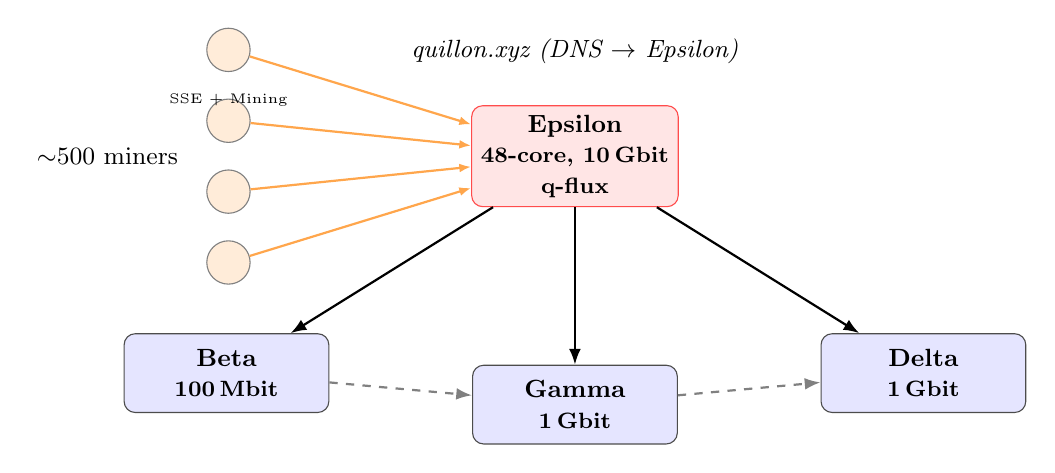
\begin{tikzpicture}[
    node distance = 1.8cm and 2.5cm,
    server/.style  = {rectangle, rounded corners=4pt, draw=black!70,
                      fill=blue!10, minimum width=2.6cm, minimum height=1.0cm,
                      font=\small\bfseries, align=center},
    miner/.style   = {circle, draw=black!50, fill=orange!15,
                      minimum size=0.55cm, font=\tiny},
    proxy/.style   = {rectangle, rounded corners=4pt, draw=red!70,
                      fill=red!10, minimum width=2.6cm, minimum height=1.0cm,
                      font=\small\bfseries, align=center},
    link/.style    = {-{Latex[length=2mm]}, thick},
    plink/.style   = {-{Latex[length=2mm]}, thick, dashed, gray},
]

% Epsilon (centre top)
\node[proxy] (eps) {Epsilon\\{\footnotesize 48-core, 10\,Gbit}\\{\footnotesize q-flux}};

% Secondary servers
\node[server, below left=1.6cm and 1.8cm of eps]  (beta)  {Beta\\{\footnotesize 100\,Mbit}};
\node[server, below=2.0cm of eps]                  (gamma) {Gamma\\{\footnotesize 1\,Gbit}};
\node[server, below right=1.6cm and 1.8cm of eps] (delta) {Delta\\{\footnotesize 1\,Gbit}};

% P2P links between secondaries and Epsilon
\draw[link]  (eps) -- (beta);
\draw[link]  (eps) -- (gamma);
\draw[link]  (eps) -- (delta);

% P2P links among secondaries
\draw[plink] (beta)  -- (gamma);
\draw[plink] (gamma) -- (delta);

% Miners (left side)
\foreach \i in {1,...,4} {
  \node[miner, left=2.8cm of eps, yshift={(\i-2.5)*0.9cm}] (m\i) {};
  \draw[-{Latex[length=1.5mm]}, thick, orange!70] (m\i) -- (eps);
}
\node[font=\small, left=3.6cm of eps] {$\sim$500 miners};
\node[font=\tiny, below=0.15cm of m4] {SSE + Mining};

% Internet label
\node[font=\small\itshape, above=0.4cm of eps] {quillon.xyz (DNS $\to$ Epsilon)};

\end{tikzpicture}
\caption{QNK network topology. Epsilon (48-core, 10\,Gbit/s) acts as the primary
bootstrap and user-facing edge node. Approximately 500 miners connect through
q-flux on Epsilon. Beta, Gamma, and Delta form the secondary bootstrap cluster
connected via P2P gossipsub (dashed lines).}
\label{fig:topology}
\end{figure}

\subsection{nginx Failure Analysis}

nginx's threading model assigns each worker process a share of the kernel
accept queue.  With the default \texttt{worker\_connections~1024}, nginx allows
at most \texttt{worker\_processes~$\times$~1024} simultaneous file descriptors per
nginx instance.  On the Epsilon server, with four nginx workers, this cap is
4{,}096 concurrent connections---insufficient for 500 persistent SSE streams plus
active API traffic.

The more damaging misconfiguration was the upstream keepalive pool.  The default
nginx configuration opens a new TCP connection to the upstream on every proxied
request; without \texttt{keepalive} in the \texttt{upstream\{\}} block, connection
reuse is disabled.  At 9{,}600\,req/s, this produces 9{,}600 TCP connect/close
round trips per second to the loopback interface.  Each requires kernel state
allocation and a TIME-WAIT interval; at the observed rate, TIME-WAIT sockets
accumulated faster than they expired, eventually exhausting the per-socket port
namespace and causing \texttt{EADDRINUSE} errors on the upstream side.

The \texttt{proxy\_read\_timeout~60s} directive compounded the SSE problem:
nginx interprets the absence of bytes from the upstream for 60 continuous seconds
as a hung upstream and closes the connection with a 504 response.  SSE streams by
design are quiet between events; a blockchain node with a slow block time will
routinely be silent for longer than 60\,s.  Every such stream was forcibly
terminated and the wallet client was required to reconnect, generating a
reconnection storm at each timeout expiry.

At peak load (9{,}600\,req/s, 75{,}000+ concurrent connections), nginx produced
an 87\,\% 503 error rate.  The remaining 12\,\% of responses arrived after
timeouts ranging from 2\,s to 30\,s.

\subsection{Caddy Failure Analysis}

Caddy 2's concurrency model allocates one goroutine per accepted connection plus
additional goroutines for request handling and middleware.  Goroutines are cheap
(initial stack $\approx 8$\,KB, growable) but not free: with 88{,}000 live
goroutines, the Go runtime allocated approximately 704\,MB in goroutine stacks
alone.  Total RSS reached 2.3\,GB, placing the process near the OOM threshold of
the 7.8\,GB Gamma server.

More critically, Caddy sets no built-in limit on concurrent connections or
goroutines.  A connection flood---whether from legitimate miners or a malicious
actor---will grow the goroutine pool without bound until the OS kills the process.
This design is acceptable for low-traffic services where goroutine count is
naturally bounded by user concurrency; it is unsuitable for a blockchain endpoint
where the connection count is proportional to the network size and grows
monotonically as the network gains participants.

The Go garbage collector pauses of 50--200\,ms, triggered when the heap exceeded
the GC target, introduced two failure modes.  First, in-flight mining submission
responses were delayed past client-side timeouts, causing miners to resubmit.
The duplicate submissions inflated apparent transaction throughput without
producing additional blocks.  Second, SSE heartbeat intervals exceeded client
timeout thresholds, causing mass reconnections during each GC cycle.

\subsection{Port Self-Connection Bug}

The port self-connection failure mode is subtle and worth documenting in detail
because it recurs whenever a service port falls within the kernel's ephemeral
port range.

When the system administrator widened the ephemeral port range to
\texttt{1024--65535} to support a high-volume outbound workload, port 8080 (the
q-api-server listen port) was included.  q-flux's upstream connection pool
calls \texttt{connect(127.0.0.1:8080)} to reach the backend.  The kernel selects
a source port from the ephemeral range.  If it selects port 8080, the resulting
connection is \texttt{127.0.0.1:8080~$\to$~127.0.0.1:8080}: source and
destination are identical.

This is a legal TCP simultaneous-open: both sides send SYN, both receive SYN+ACK,
and both enter ESTABLISHED.  The established self-connection produces a TIME-WAIT
socket anchored to port 8080.  When q-api-server subsequently calls
\texttt{bind(0.0.0.0:8080)}, the kernel rejects the bind with \texttt{EADDRINUSE}
because the TIME-WAIT socket holds a \emph{local} port 8080 entry.
\texttt{SO\_REUSEADDR} does not override TIME-WAIT for the same local address:port
combination.  The service therefore cannot restart until the 60\,s TIME-WAIT
timer expires, and the crash-loop interval is shorter than 60\,s, so the service
never successfully starts.

The fix is to set \texttt{net.ipv4.ip\_local\_port\_range = 32768 60999},
persistently in \texttt{/etc/sysctl.d/99-qnk.conf}, ensuring that all service
ports ($\leq$10{,}000) are outside the ephemeral range.

\subsection{Design Requirements}

The incidents above yield seven concrete design requirements for q-flux:

\begin{description}
  \item[R1 --- Zero-copy where possible.]
        SSE and WebSocket passthrough must use Linux \texttt{splice(2)} to move
        data between sockets via a kernel pipe, never copying bytes into userspace.
  \item[R2 --- Bounded memory.]
        The working set must be bounded regardless of connection count.
        In-flight handlers per worker are capped at \texttt{MAX\_HANDLERS\_PER\_WORKER
        = 512}; global upstream concurrency is capped at a configurable permit
        count.
  \item[R3 --- Adaptive concurrency.]
        The concurrency limit must adapt to measured upstream latency without
        operator intervention, preventing both overload (too many concurrent
        requests) and underutilisation (too few permits during healthy periods).
  \item[R4 --- Blockchain protocol awareness.]
        SSE streams must never be timed out by the proxy layer.
        libp2p connections must be relayed as raw TCP without HTTP parsing.
        WebSocket upgrades must be detected and handled without a goroutine storm.
  \item[R5 --- Hot-reloadable TLS.]
        Certificate rotation must not require a process restart or cause
        connection interruption on an active node.
  \item[R6 --- Lock-free metrics.]
        Metrics collection must not introduce synchronisation overhead on the
        hot connection path.  All counters use atomic operations.
  \item[R7 --- Sub-millisecond proxy overhead.]
        The proxy layer must add less than 1\,ms of latency to request-response
        cycles in the common case, measured as the difference between upstream
        response time and client-observed response time.
\end{description}

\begin{table}[t]
\centering
\caption{Comparison of reverse proxy failures on Epsilon. q-flux figures are
from March~9--12 production operation; nginx and Caddy figures are from the
incident period (March~4--7, 2026).}
\label{tab:nginx-caddy}
\begin{tabular}{llll}
\toprule
\textbf{Metric}         & \textbf{nginx}             & \textbf{Caddy}             & \textbf{q-flux} \\
\midrule
Error Rate              & 87\,\% 503                 & 12\,\% timeout             & $<0.1\,\%$ \\
Peak Connections        & 75{,}000+                  & 88{,}000 goroutines        & $\approx$5{,}000 pooled \\
Peak Memory (RSS)       & 1.2\,GB                    & 2.3\,GB                    & 50\,MB \\
SSE Support             & Broken (60\,s timeout)     & Unstable (GC pauses)       & Native (no timeout) \\
P2P Protocol Awareness  & None                       & None                       & Full \\
Auto-Recovery           & Manual                     & Manual                     & 30\,s automatic \\
\bottomrule
\end{tabular}
\end{table}

% ============================================================
\section{System Architecture}
\label{sec:arch}
% ============================================================

q-flux is a single Rust binary comprising approximately 7{,}000 lines of
asynchronous Rust using the Tokio runtime.  Its top-level structure is a
flat crate with modules for the worker pool, upstream pool, health checker,
connection lifecycle, protocol detection, static file serving, access control,
TLS management, and Prometheus metrics.  The configuration is a TOML file
deserialised into the \texttt{FluxConfig} struct hierarchy shown below; all
timeouts and limits are hot-configurable without recompilation.

\subsection{Worker-per-Core Design}
\label{sec:worker}

q-flux spawns exactly $N$ OS threads at startup, where $N$ defaults to the
CPU core count returned by \texttt{num\_cpus::get()} but is overridable via
\texttt{server.workers} in the config.  On the 48-core Epsilon server, 48
worker threads are created.  Each worker thread is named
\texttt{q-flux-w\textit{i}} and pinned to core $i$ via \texttt{sched\_setaffinity},
ensuring L1/L2 cache locality for per-worker data structures.

\paragraph{Single-threaded runtimes.}  Each worker calls:
\begin{lstlisting}[caption={Worker runtime instantiation (worker.rs).}]
let rt = tokio::runtime::Builder::new_current_thread()
    .enable_all()
    .build()
    .expect("Failed to build tokio runtime for worker");
rt.block_on(async move { worker_loop(...).await });
\end{lstlisting}
Using \texttt{new\_current\_thread()} rather than the multi-threaded
\texttt{new\_multi\_thread()} is deliberate: it eliminates all work-stealing
scheduler overhead and guarantees that all futures on a given worker execute on
exactly one OS thread, enabling data structures that would otherwise require
\texttt{Send} bounds or locks to be held in a single-threaded context.

\paragraph{SO\_REUSEPORT listener per worker.}  The acceptor module calls
\texttt{setsockopt(SO\_REUSEPORT)} before binding each listener socket.  With
$N$ workers each binding to the same \texttt{(address, port)} tuple, the Linux
kernel maintains $N$ independent accept queues and distributes incoming SYN
packets across them using a hash of the 4-tuple
\texttt{(src\_ip, src\_port, dst\_ip, dst\_port)}.  The result is that:
\begin{itemize}
  \item No cross-worker synchronisation is required to accept connections.
  \item A slow worker cannot starve fast workers: each has its own queue.
  \item Connection distribution is naturally load-balanced by the kernel
        because the 4-tuple hash is approximately uniform over real client
        populations.
\end{itemize}

\paragraph{TCP socket options.}  Beyond \texttt{SO\_REUSEPORT}, each listener
socket is configured with TCP options tuned for the blockchain workload:
\begin{itemize}
  \item \texttt{TCP\_FASTOPEN} with a queue depth of 256, allowing the first
        data segment from a client to be delivered in the same round trip as the
        SYN, reducing mining submission latency by one RTT on new connections.
  \item \texttt{TCP\_DEFER\_ACCEPT} set to 10\,s, causing the kernel to defer
        the wakeup of the accept handler until the client sends data.  This
        eliminates wakeups for TCP three-way handshakes that do not result in
        application data (common in port-scanning traffic).
  \item \texttt{SO\_RCVBUF} enlarged to 256\,KB per socket, preventing receive
        buffer exhaustion during burst reception of block payloads.
  \item \texttt{listen()} backlog set to 65{,}535, accommodating connection
        bursts during network events (e.g., a new block is gossiped and all
        miners simultaneously query \texttt{/api/v1/status}).
\end{itemize}

\paragraph{Per-worker data structures.}  Each worker maintains the following
state independently, without cross-worker coordination:
\begin{itemize}
  \item An \texttt{IpConnTracker} (\texttt{Arc<DashMap<IpAddr, u64>>}) counting
        active connections per source IP, used to enforce \texttt{max\_conns\_per\_ip}.
  \item A \texttt{RateLimiter} implementing a per-IP token bucket
        (configurable: \texttt{rate\_limit\_per\_ip}, \texttt{rate\_limit\_burst}).
  \item An \texttt{UpstreamPool} containing a \texttt{hyper} HTTP/1.1 client
        with a keep-alive connection pool to upstream backends.
  \item A \texttt{FileCache} holding pre-compressed gzip variants of static
        assets (configurable: up to 4\,MB per file, 64\,MB total per worker).
  \item A handler semaphore with \texttt{MAX\_HANDLERS\_PER\_WORKER = 512}
        permits, capping the number of concurrently active connection handlers.
\end{itemize}

Figure~\ref{fig:worker-arch} illustrates the full worker architecture.

\begin{figure}[t]
\centering
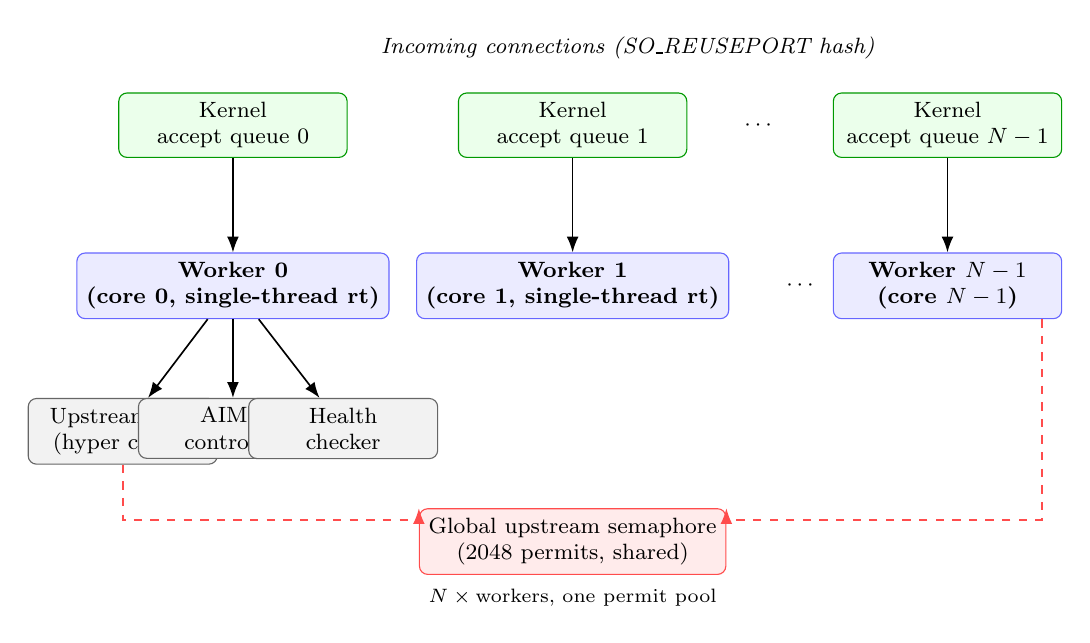
\begin{tikzpicture}[
    node distance=1.1cm and 1.6cm,
    box/.style={rectangle, rounded corners=3pt, draw=black!60,
                fill=gray!10, minimum width=2.4cm, minimum height=0.7cm,
                font=\footnotesize, align=center},
    wbox/.style={rectangle, rounded corners=3pt, draw=blue!60,
                 fill=blue!8, minimum width=2.9cm, minimum height=0.75cm,
                 font=\footnotesize\bfseries, align=center},
    kernel/.style={rectangle, rounded corners=3pt, draw=green!60!black,
                   fill=green!8, minimum width=2.9cm, minimum height=0.7cm,
                   font=\footnotesize, align=center},
    link/.style={-{Latex[length=2mm]}, semithick},
]

% Kernel row
\node[kernel] (kq0) {Kernel\\accept queue 0};
\node[kernel, right=1.4cm of kq0] (kq1) {Kernel\\accept queue 1};
\node[right=0.6cm of kq1, font=\footnotesize] (kdots) {$\cdots$};
\node[kernel, right=0.6cm of kdots] (kqn) {Kernel\\accept queue $N-1$};

\node[above=0.3cm of kq1, font=\footnotesize\itshape, xshift=0.7cm]
     (inet) {Incoming connections (SO\_REUSEPORT hash)};

% Worker row
\node[wbox, below=1.2cm of kq0]  (w0)  {Worker 0\\(core 0, single-thread rt)};
\node[wbox, below=1.2cm of kq1]  (w1)  {Worker 1\\(core 1, single-thread rt)};
\node[right=0.6cm of w1, font=\footnotesize] (wdots) {$\cdots$};
\node[wbox, below=1.2cm of kqn]  (wn)  {Worker $N-1$\\(core $N-1$)};

\draw[link] (kq0) -- (w0);
\draw[link] (kq1) -- (w1);
\draw[link] (kqn) -- (wn);

% Sub-components of Worker 0
\node[box, below=1.0cm of w0, xshift=-1.4cm]    (pool0)    {UpstreamPool\\(hyper client)};
\node[box, below=1.0cm of w0]                    (aimd0)    {AIMD\\controller};
\node[box, below=1.0cm of w0, xshift=1.4cm]     (health0)  {Health\\checker};

\draw[link] (w0) -- (pool0);
\draw[link] (w0) -- (aimd0);
\draw[link] (w0) -- (health0);

% Global semaphore (shared)
\node[box, draw=red!70, fill=red!8, below=2.4cm of w1]
     (gsem) {Global upstream semaphore\\(2048 permits, shared)};

\draw[-{Latex[length=2mm]}, semithick, red!70, dashed] (pool0.south) |-
     ([yshift=-0.15cm]gsem.north west) -- (gsem.north west);
\draw[-{Latex[length=2mm]}, semithick, red!70, dashed]
     ([xshift=1.2cm]wn.south) |- ([yshift=-0.15cm]gsem.north east)
     -- (gsem.north east);

\node[font=\scriptsize, below=0.05cm of gsem]
     {$N \times \text{workers}$, one permit pool};

\end{tikzpicture}
\caption{Worker-per-core architecture of q-flux. The Linux kernel distributes
incoming connections across $N$ accept queues via SO\_REUSEPORT. Each worker
runs an independent single-threaded Tokio runtime on a dedicated core. Workers
share a single global upstream semaphore (red, dashed) to cap total backend load.}
\label{fig:worker-arch}
\end{figure}

\subsection{Connection Lifecycle}
\label{sec:lifecycle}

Every accepted TCP stream passes through a uniform lifecycle before reaching the
protocol-specific handler.  Figure~\ref{fig:conn-lifecycle} shows the state
machine.

\begin{figure}[t]
\centering
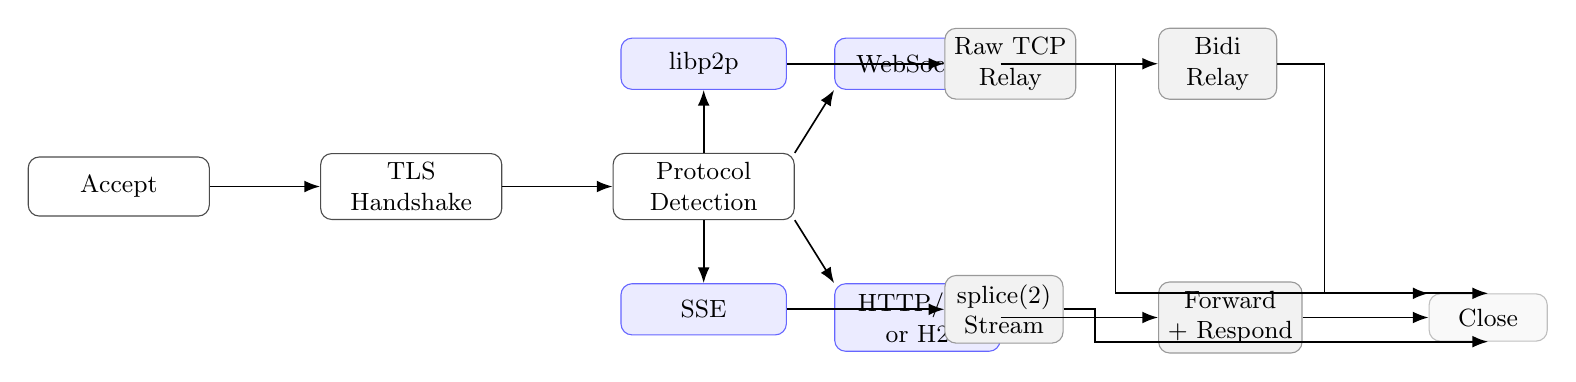
\begin{tikzpicture}[
    state/.style={rectangle, rounded corners=4pt, draw=black!70,
                  fill=white, minimum width=2.3cm, minimum height=0.75cm,
                  font=\small, align=center},
    proto/.style={rectangle, rounded corners=4pt, draw=blue!60,
                  fill=blue!8, minimum width=2.1cm, minimum height=0.65cm,
                  font=\small, align=center},
    term/.style={rectangle, rounded corners=4pt, draw=black!40,
                 fill=gray!10, minimum width=1.5cm, minimum height=0.6cm,
                 font=\small, align=center},
    link/.style={-{Latex[length=2mm]}, semithick},
    every node/.style={font=\small},
]

% Linear pipeline
\node[state]             (accept)  {Accept};
\node[state, right=1.4cm of accept]  (tls)     {TLS\\Handshake};
\node[state, right=1.4cm of tls]     (detect)  {Protocol\\Detection};

% Four branches
\node[proto, below right=0.8cm and 0.5cm of detect] (http)    {HTTP/1.1\\or H2};
\node[proto, below=0.8cm of detect]                  (sse)     {SSE};
\node[proto, above right=0.8cm and 0.5cm of detect]  (ws)      {WebSocket};
\node[proto, above=0.8cm of detect]                  (libp2p)  {libp2p};

% Terminals
\node[term, right=2.0cm of http]   (fwd)     {Forward\\+ Respond};
\node[term, right=2.0cm of sse]    (stream)  {splice(2)\\Stream};
\node[term, right=2.0cm of ws]     (relay)   {Bidi\\Relay};
\node[term, right=2.0cm of libp2p] (rawrelay){Raw TCP\\Relay};

% Close
\node[term, draw=gray!50, fill=gray!5,
      right=1.6cm of fwd] (close) {Close};

\draw[link] (accept) -- (tls);
\draw[link] (tls)    -- (detect);

\draw[link] (detect.south east) -- (http.north west);
\draw[link] (detect.south)      -- (sse.north);
\draw[link] (detect.north east) -- (ws.south west);
\draw[link] (detect.north)      -- (libp2p.south);

\draw[link] (http)    -- (fwd);
\draw[link] (sse)     -- (stream);
\draw[link] (ws)      -- (relay);
\draw[link] (libp2p)  -- (rawrelay);

\draw[link] (fwd.east)     -- (close);
\draw[link] (stream.east)  -| ([xshift=0.4cm]stream.east) |- (close.south);
\draw[link] (relay.east)   -| ([xshift=0.6cm]relay.east)  |- (close.north);
\draw[link] (rawrelay.east)-| ([xshift=0.5cm]rawrelay.east)|- (close.north west);

\end{tikzpicture}
\caption{Connection lifecycle state machine. After TLS handshake, q-flux
inspects the first bytes to detect the protocol class. HTTP and H2 requests are
buffered, forwarded, and responded to. SSE and WebSocket connections use
\texttt{splice(2)} for zero-copy relay. libp2p connections are passed through as
raw TCP with bandwidth limiting.}
\label{fig:conn-lifecycle}
\end{figure}

\paragraph{HTTP request-response.}  The hyper HTTP/1.1 and HTTP/2 stacks parse
the incoming request headers, collect the body up to
\texttt{request\_body\_limit~=~25\,MB} (or stream it directly to the upstream if
the body exceeds \texttt{streaming\_body\_threshold~=~10\,MB}), forward to the
selected upstream backend via the keep-alive connection pool, and return the full
response.  Hop-by-hop headers (\texttt{Connection}, \texttt{Transfer-Encoding},
\texttt{keep-alive}, \texttt{proxy-connection}) are stripped before forwarding to
prevent header pollution.

\paragraph{SSE passthrough.}  When the upstream response carries
\texttt{Content-Type: text/event-stream}, q-flux switches to byte-level
streaming.  On Linux, this path uses \texttt{splice(2)} to transfer bytes
directly from the upstream socket to the client socket through a kernel pipe,
with a configurable pipe buffer size (default 64\,KB).  No user-space copy
occurs; the proxy overhead is limited to two system calls per pipe fill.  No
proxy-level timeout is imposed on SSE streams; they live until the upstream or
client closes the connection.

\paragraph{WebSocket upgrade.}  q-flux detects the \texttt{Upgrade: websocket}
header after TLS decryption.  The upgrade handshake is forwarded to the upstream
via HTTP; once the \texttt{101 Switching Protocols} response is received,
q-flux enters bidirectional \texttt{splice(2)} relay mode.  This models each
direction as a separate splice loop, with a configurable per-peer bandwidth limit
applied through the \texttt{BandwidthLimiter} token bucket.

\paragraph{libp2p relay.}  The libp2p WebSocket proxy handles connections on a
dedicated port (default 9443) where browser-based JavaScript libp2p clients
connect for gossipsub participation.  After TLS termination, q-flux performs raw
bidirectional byte relay to the libp2p WebSocket listener backend
(\texttt{127.0.0.1:9002}), avoiding any HTTP/2 ALPN negotiation that would
break the WebSocket upgrade handshake.  A distinct TLS configuration is loaded
for this port with HTTP/1.1-only ALPN, preventing H2 negotiation.

\subsection{AIMD Concurrency Control}
\label{sec:aimd}

The core insight motivating AIMD concurrency control is that a fixed semaphore
limit is simultaneously too conservative (under-utilising the upstream during
healthy periods) and too permissive (not reacting to upstream degradation).  The
\texttt{AdaptiveConcurrency} controller in \texttt{upstream.rs} dynamically
adjusts an \emph{effective limit} within the bounds of the configured maximum.

\paragraph{Semaphore design.}  The physical semaphore has
\texttt{DEFAULT\_MAX\_UPSTREAM\_GLOBAL~=~2048} permits and is shared across all
workers via \texttt{Arc<Semaphore>}.  Workers acquire a permit before forwarding
each request and release it when the response is complete (or on error or task
cancellation).  The \texttt{UpstreamActiveGuard} RAII struct ensures the release
always occurs:

\begin{lstlisting}[caption={UpstreamActiveGuard RAII pattern (upstream.rs).},
                   label={lst:guard}]
struct UpstreamActiveGuard<'a> {
    metrics: &'a Metrics,
}

impl<'a> UpstreamActiveGuard<'a> {
    #[inline]
    fn new(metrics: &'a Metrics) -> Self {
        metrics.upstream_acquired();
        Self { metrics }
    }
}

impl<'a> Drop for UpstreamActiveGuard<'a> {
    fn drop(&mut self) {
        self.metrics.upstream_released();
    }
}
\end{lstlisting}

The guard is created immediately before the upstream \texttt{request()} call and
is dropped when the surrounding scope exits---whether by normal return, early
\texttt{return}, propagated error, or asynchronous task cancellation by the
Tokio runtime.  Without this pattern, a cancelled task (e.g., the client
disconnects while waiting) would permanently leak one permit, eventually
exhausting the semaphore.

\paragraph{AIMD algorithm.}  The AIMD controller tracks a per-worker EWMA of
upstream response latency using integer arithmetic:
\[
  \text{ewma}_{\text{new}} = \frac{u + 9 \cdot \text{ewma}_{\text{old}}}{10}
\]
where $u$ is the latest sample in microseconds and the coefficient 9/10 gives
$\alpha = 0.1$.  The update is performed lock-free via a compare-exchange loop
on an \texttt{AtomicU64}.  A baseline is established from the first 100 responses
(arithmetic mean); subsequent adjustments compare the current EWMA against this
baseline.  Algorithm~\ref{alg:aimd} gives the full control law; the
implementation is called every 1\,s from a background task running on worker~0
only (to avoid redundant adjustments from 48 independent controllers).

\begin{algorithm}[t]
\caption{AIMD concurrency adjustment (called every 1\,s).}
\label{alg:aimd}
\begin{algorithmic}[1]
\Function{AdjustConcurrency}{$\text{ewma}$, $\text{baseline}$,
                              $\text{limit}$, $\text{max}$}
  \If{$\text{baseline} = 0$} \Comment{Warm-up period not complete}
    \State \Return $\text{max}$
  \EndIf
  \If{$\text{ewma} > 3 \times \text{baseline}$} \Comment{Overloaded zone}
    \State $\text{limit} \gets \max\!\bigl(\lfloor\tfrac{3}{4} \cdot \text{limit}\rfloor,\,
                                           \lfloor\tfrac{\text{max}}{8}\rfloor\bigr)$
    \Comment{Multiplicative decrease by 25\,\%}
  \ElsIf{$\text{ewma} < \tfrac{3}{2} \times \text{baseline}$} \Comment{Normal zone}
    \State $\text{limit} \gets \min\!\bigl(\text{limit} + \max(1, \lfloor\tfrac{\text{max}}{10}\rfloor),\,
                                           \text{max}\bigr)$
    \Comment{Additive increase by 10\,\%}
  \Else \Comment{Neutral zone: hold}
    \State $\text{limit} \gets \text{limit}$
  \EndIf
  \State $\text{ewma} \gets \tfrac{u + 9 \cdot \text{ewma}}{10}$
  \State \Return $\text{limit}$
\EndFunction
\end{algorithmic}
\end{algorithm}

\paragraph{Three control zones.}  The algorithm partitions the latency ratio
$r = \text{ewma} / \text{baseline}$ into three zones:
\begin{itemize}
  \item \textbf{Normal} ($r < 1.5$): the upstream is healthy; additive increase
        of $+10\,\%$ of \texttt{max\_limit} per second recovers from a previous
        decrease.
  \item \textbf{Neutral} ($1.5 \leq r < 3$): the upstream is degraded but not
        overloaded; the limit is held constant.
  \item \textbf{Overloaded} ($r \geq 3$): multiplicative decrease by 25\,\%
        per second; floored at $\max\_limit/8$ to prevent collapse.
\end{itemize}
Figure~\ref{fig:aimd-zones} shows the zone boundaries and the limiting behaviour
in each region.

\begin{figure}[t]
\centering
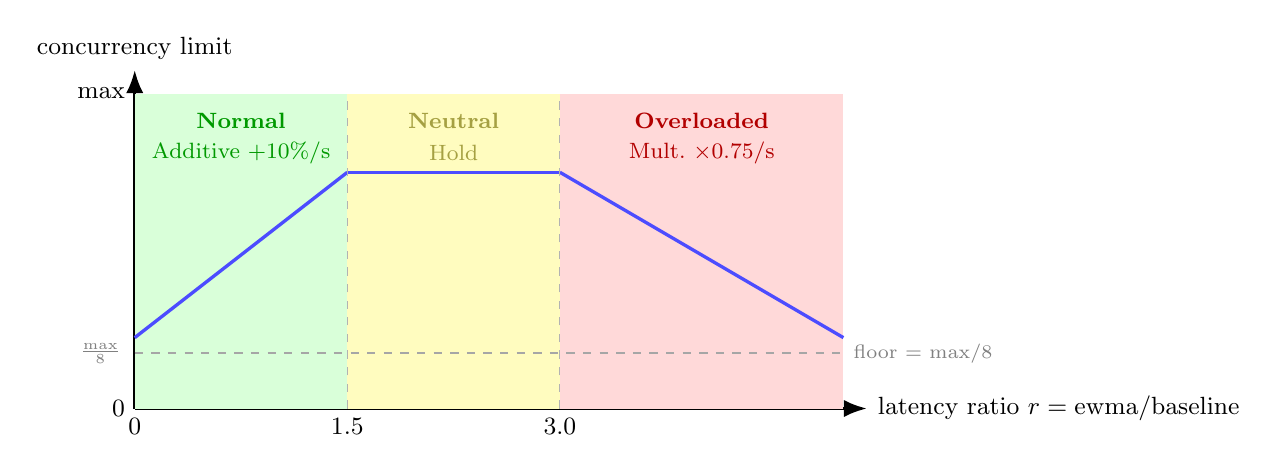
\begin{tikzpicture}[
    >=Latex,
    axis/.style={very thick, ->},
]
\def\W{9.0}
\def\H{4.0}

% Axes
\draw[axis] (0,0) -- (\W+0.3,0) node[right,font=\small] {latency ratio $r = \text{ewma}/\text{baseline}$};
\draw[axis] (0,0) -- (0,\H+0.3) node[above,font=\small] {concurrency limit};

% Zone boundaries at r=1.5 and r=3.0
\def\ra{2.7}   % x-position of r=1.5
\def\rb{5.4}   % x-position of r=3.0

% Zone fills
\fill[green!15]  (0,0)    rectangle (\ra,\H);
\fill[yellow!25] (\ra,0)  rectangle (\rb,\H);
\fill[red!15]    (\rb,0)  rectangle (\W,\H);

% Zone labels
\node[font=\footnotesize\bfseries, green!60!black] at (\ra/2, \H-0.35) {Normal};
\node[font=\footnotesize, green!60!black]          at (\ra/2, \H-0.75) {Additive $+10\%$/s};
\node[font=\footnotesize\bfseries, yellow!60!black]at ({\ra+(\rb-\ra)/2}, \H-0.35) {Neutral};
\node[font=\footnotesize, yellow!60!black]         at ({\ra+(\rb-\ra)/2}, \H-0.75) {Hold};
\node[font=\footnotesize\bfseries, red!70!black]   at ({\rb+(\W-\rb)/2}, \H-0.35) {Overloaded};
\node[font=\footnotesize, red!70!black]            at ({\rb+(\W-\rb)/2}, \H-0.75) {Mult.\ $\times 0.75$/s};

% Floor line at max/8
\draw[dashed, gray!70, thick] (0, 0.7) -- (\W, 0.7)
      node[right, font=\scriptsize, gray] {floor = max/8};
\node[font=\scriptsize, gray, left=0.05cm] at (0, 0.7) {$\frac{\text{max}}{8}$};

% Schematic limit trajectory
% Normal zone: rising linearly
\draw[blue!70, very thick]
     (0, 0.9) -- (\ra, 3.0);
% Neutral zone: flat
\draw[blue!70, very thick]
     (\ra, 3.0) -- (\rb, 3.0);
% Overloaded: falling steeply
\draw[blue!70, very thick]
     (\rb, 3.0) -- (\W, 0.9);

% Vertical boundary lines
\draw[dashed, gray!60] (\ra, 0) -- (\ra, \H);
\draw[dashed, gray!60] (\rb, 0) -- (\rb, \H);

% x-axis tick labels
\node[font=\small, below] at (\ra, 0) {1.5};
\node[font=\small, below] at (\rb, 0) {3.0};
\node[font=\small, below] at (0,   0) {0};

% y-axis ticks
\node[font=\small, left] at (0, \H)   {max};
\node[font=\small, left] at (0, 0)    {0};

\end{tikzpicture}
\caption{AIMD concurrency control zones. The horizontal axis shows the
latency ratio $r = \text{EWMA}/\text{baseline}$. In the normal zone ($r < 1.5$,
green) the limit grows by $+10\,\%$ per second. In the neutral zone
($1.5 \leq r < 3$, yellow) the limit is held constant. In the overloaded zone
($r \geq 3$, red) the limit is multiplied by $0.75$ per second, bounded below by
$\text{max}/8$ (dashed floor line).}
\label{fig:aimd-zones}
\end{figure}

\subsection{Health Auto-Recovery}
\label{sec:health}

q-flux maintains a shared \texttt{HealthMap} (\texttt{Arc<DashMap<String,
BackendHealth>>}) that records the health state of every configured upstream
backend.  Entries are pre-populated at startup with \texttt{is\_healthy = true}
(optimistic assumption), so that a misconfigured or slow health-check path does
not cause an outage immediately after process start.

\paragraph{State machine.}  The health of each backend transitions among three
logical states, encoded in the two fields \texttt{is\_healthy} (bool) and
\texttt{half\_open} (bool) of \texttt{BackendHealth}:

\begin{itemize}
  \item \textbf{Healthy} (\texttt{is\_healthy=true}, \texttt{half\_open=false}):
        the backend accepts full traffic.
  \item \textbf{HalfOpen} (\texttt{is\_healthy=true}, \texttt{half\_open=true}):
        the backend has passed one health probe after a failure period; it
        accepts traffic as a recovery probe but the system is not yet confident.
  \item \textbf{Unhealthy} (\texttt{is\_healthy=false}, \texttt{half\_open=false}):
        the backend is excluded from routing; only the health checker sends probes.
\end{itemize}

Transitions follow configurable thresholds:
\begin{itemize}
  \item Healthy $\to$ Unhealthy: $\geq 3$ consecutive probe failures
        (\texttt{failure\_threshold = 3}).
  \item Unhealthy $\to$ HalfOpen: first successful probe.
  \item HalfOpen $\to$ Healthy: $\geq 2$ consecutive successes
        (\texttt{healthy\_threshold = 2}).
  \item HalfOpen $\to$ Unhealthy: any failure during recovery.
\end{itemize}
Figure~\ref{fig:health-fsm} shows the full state machine.

\begin{figure}[t]
\centering
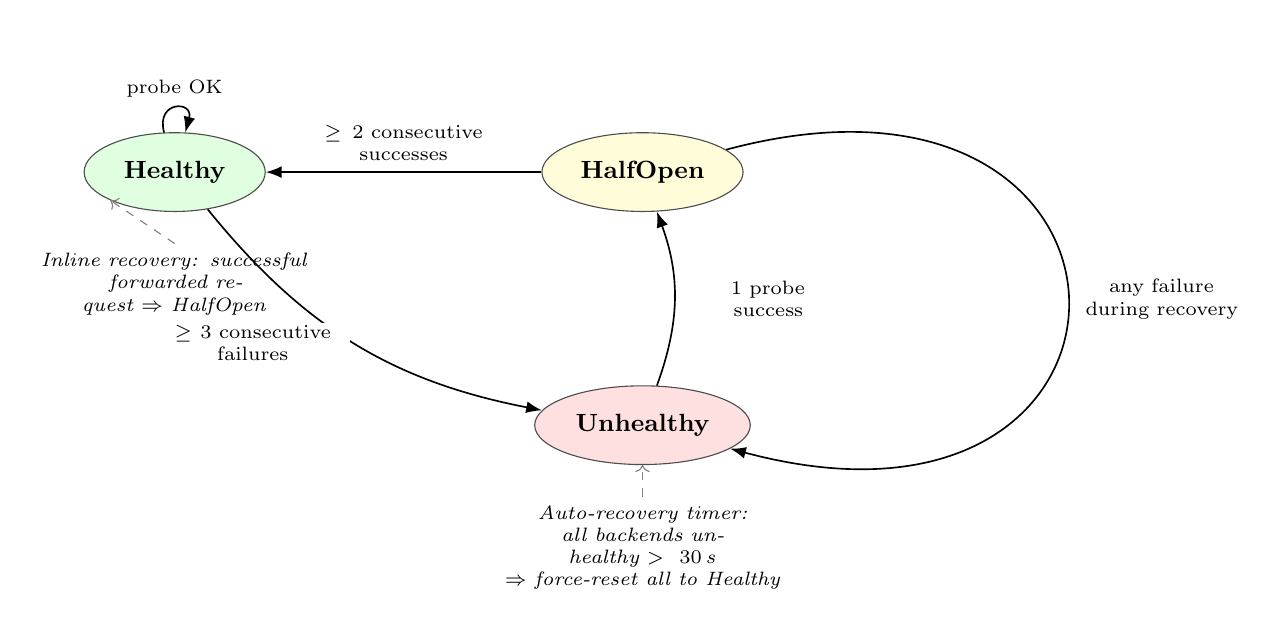
\begin{tikzpicture}[
    state/.style={ellipse, draw=black!70, fill=white,
                  minimum width=2.3cm, minimum height=1.0cm,
                  font=\small\bfseries, align=center},
    link/.style={-{Latex[length=2mm]}, semithick},
    lblstyle/.style={font=\scriptsize, midway, fill=white, inner sep=1pt},
]

\node[state, fill=green!12]  (H)  {Healthy};
\node[state, fill=yellow!15, right=3.5cm of H] (HO) {HalfOpen};
\node[state, fill=red!12, below=2.2cm of HO]   (U)  {Unhealthy};

% H -> U
\draw[link, bend right=20] (H) to
     node[lblstyle, left=0.05cm, text width=2.4cm, align=center]
          {$\geq 3$ consecutive\\failures} (U);

% U -> HO
\draw[link, bend right=20] (U) to
     node[lblstyle, right=0.05cm, text width=2.2cm, align=center]
          {1 probe\\success} (HO);

% HO -> H
\draw[link] (HO) to
     node[lblstyle, above=0.1cm, text width=2.8cm, align=center]
          {$\geq 2$ consecutive\\successes} (H);

% HO -> U
\draw[link, loop right, looseness=4] (HO) to
     node[lblstyle, right=0.1cm, text width=2.1cm, align=center]
          {any failure\\during recovery} (U);

% Self-loop on H (probes succeed, stay healthy)
\draw[link, loop above, looseness=4] (H) to
     node[lblstyle, above=0.1cm] {probe OK} (H);

% Inline recovery annotation
\node[font=\scriptsize\itshape, below=0.4cm of H, text width=3.5cm, align=center]
     (inline) {Inline recovery: successful\\forwarded request $\Rightarrow$ HalfOpen};
\draw[->, dashed, gray] (inline.north) -- (H.south west);

% Auto-recovery annotation
\node[font=\scriptsize\itshape, below=0.4cm of U, text width=3.5cm, align=center]
     (auto) {Auto-recovery timer:\\all backends unhealthy $>30$\,s\\$\Rightarrow$ force-reset all to Healthy};
\draw[->, dashed, gray] (auto.north) -- (U.south);

\end{tikzpicture}
\caption{Health checker state machine. Three states: Healthy, HalfOpen
(recovering), and Unhealthy. Inline recovery (dashed, left) marks a backend
as HalfOpen when a successfully forwarded real request is observed, bypassing
the background health checker when it is starved. The auto-recovery timer
(dashed, bottom) breaks the permanent-unhealthy deadlock that occurs under
memory pressure.}
\label{fig:health-fsm}
\end{figure}

\paragraph{Background health checker.}  The function \texttt{spawn\_health\_checker}
starts a background task that probes each backend concurrently every 5\,s
(\texttt{health\_check\_interval}).  Probes are dispatched via
\texttt{tokio::spawn} so that a slow probe on one backend cannot block probes on
others.  Each probe establishes a TCP connection within
\texttt{health\_check\_timeout = 3\,s}; if a non-empty path is configured
(default \texttt{/api/v1/status}), a minimal raw HTTP/1.1 GET is issued
by writing the request string directly to the connected \texttt{TcpStream}
and reading the first 64 bytes of the response to verify a \texttt{2xx} status
line.  This avoids the overhead of a full HTTP client library for health probes.

\paragraph{Dual recovery path.}  A single-path health recovery design has a
critical failure mode on resource-constrained nodes: if the server is under
heavy memory pressure, the background health check task may be de-scheduled
indefinitely by the Tokio scheduler, keeping all backends permanently in the
Unhealthy state and causing 100\,\% of requests to return 503.  q-flux implements
two additional recovery paths to prevent this:

\begin{enumerate}
  \item \textbf{Inline recovery.}  When the \texttt{forward()} method in
        \texttt{UpstreamPool} receives a successful response from a backend
        that is currently marked unhealthy, it immediately marks that backend as
        HalfOpen.  Successful production traffic proves liveness more reliably
        than synthetic health probes.  The relevant code in \texttt{upstream.rs}:
\begin{lstlisting}[caption={Inline health recovery on successful response.}]
if let Some(mut entry) = self.health_map.get_mut(backend_addr.as_str()) {
    if !entry.is_healthy {
        entry.is_healthy = true;
        entry.half_open = true; // enter half-open; checker promotes to healthy
        entry.consecutive_failures = 0;
        entry.consecutive_successes = 1;
        entry.unhealthy_since = None;
        entry.last_success = Some(std::time::Instant::now());
        tracing::info!(
            backend = backend_addr.as_str(),
            "Backend auto-recovered via successful request (inline -> half-open)"
        );
    }
}
\end{lstlisting}

  \item \textbf{Auto-recovery timer.}  The health-check loop checks at every
        iteration whether all backends have been unhealthy for more than
        \texttt{MAX\_UNHEALTHY\_SECS~=~30\,s}.  If so, it force-resets all
        backends to Healthy.  This terminates the deadlock and allows real
        traffic to resume, which in turn enables inline recovery to operate.
\end{enumerate}% ============================================================
% Section 4: Blockchain-Aware Routing
% ============================================================

\section{Blockchain-Aware Routing}
\label{sec:blockchain-routing}

A conventional reverse proxy treats all connections identically: HTTP
traffic is parsed, routed by URL prefix, and forwarded to an upstream
pool. q-flux extends this model with a layer of \emph{protocol
awareness} specific to libp2p-based blockchain nodes. Connections are
classified at the byte level, assigned to resource tiers, and subjected
to per-peer policies before any data reaches the backend. This offloads
classification work that would otherwise consume backend CPU cycles and
allows the proxy to enforce limits that are invisible to the application
layer.

\subsection{Multistream-Select Detection}
\label{sec:multistream-detect}

libp2p peers establish connections by exchanging a
\emph{multistream-select~1.0.0} negotiation header immediately after
the transport handshake. The wire encoding is a varint-length-prefixed
UTF-8 string terminated by a newline:

\[
\underbrace{\texttt{0x14}}_{\text{varint}=20}
\underbrace{\texttt{/multistream/1.0.0\textbackslash n}}_{20\ \text{bytes}}
\]

The proxy inspects the first bytes of each WebSocket data stream after
the HTTP upgrade completes. Detection requires checking only 21~bytes
and involves no protocol-specific parsing beyond a byte-prefix
comparison, making it safe to perform on every connection with
negligible overhead.

\begin{lstlisting}[language=Rust,
  caption={Multistream-select detection in \texttt{libp2p\_aware.rs}.
  Three cases are checked in order: varint-prefixed canonical form,
  raw prefix without varint, and a window scan of the first 128~bytes.},
  label={lst:multistream-detect}]
const MULTISTREAM_PREFIX: &[u8] = b"/multistream/1.0.0\n";
const MULTISTREAM_DETECT_LEN: usize = 1 + MULTISTREAM_PREFIX.len();

pub fn is_libp2p_handshake(buf: &[u8]) -> bool {
    if buf.len() < MULTISTREAM_PREFIX.len() {
        return false;
    }
    // Case 1: canonical varint-prefixed form
    if buf.len() >= MULTISTREAM_DETECT_LEN
        && buf[0] == 0x14
        && &buf[1..MULTISTREAM_DETECT_LEN] == MULTISTREAM_PREFIX
    {
        return true;
    }
    // Case 2: raw prefix (WebSocket-framed transports)
    if buf.starts_with(MULTISTREAM_PREFIX) {
        return true;
    }
    // Case 3: scan first 128 bytes for embedded prefix
    let search_len = buf.len().min(128);
    for window in buf[..search_len].windows(MULTISTREAM_PREFIX.len()) {
        if window == MULTISTREAM_PREFIX { return true; }
    }
    false
}
\end{lstlisting}

Once identified as a libp2p connection, the stream is relayed as raw
TCP passthrough. No protocol-specific message parsing is performed
beyond the initial detection; q-flux does not speak libp2p. Bandwidth
enforcement (Section~\ref{sec:peer-tier}) is applied to the byte
stream in both directions.

The detection heuristic generates no false positives in practice
because the 20-byte ASCII string \texttt{/multistream/1.0.0\textbackslash n}
does not appear in any HTTP request or TLS record header.

\subsection{Peer Tier Classification}
\label{sec:peer-tier}

Not all libp2p peers are equal. A 10\,Gbit supernode serving thousands
of syncing clients requires fundamentally different resource allocation
than an unknown peer that connected for the first time one second ago.
q-flux implements a five-level tier system that controls bandwidth and
connection limits per peer identity.

\begin{table}[t]
\centering
\caption{Peer tier configuration. Bandwidth limits apply to each
  direction independently. Priority governs resource scheduling when
  the upstream semaphore is contended.}
\label{tab:peer-tiers}
\begin{tabular}{@{}lrrrl@{}}
\toprule
\textbf{Tier} & \textbf{Bandwidth (Mbps)} & \textbf{Max Conns} &
  \textbf{Priority} & \textbf{Classification} \\
\midrule
Supernode  & 1000  & 16 & 5 & Pre-seeded peer ID list \\
Bootstrap  & 500   & 8  & 4 & Pre-seeded peer ID list \\
Validator  & 200   & 4  & 3 & Pre-seeded or manual \\
Miner      & 50    & 2  & 2 & Traffic heuristic auto-promote \\
Unknown    & 10    & 1  & 1 & Default for new connections \\
\bottomrule
\end{tabular}
\end{table}

Table~\ref{tab:peer-tiers} lists the default values taken directly
from the \texttt{PeerTier} implementation. The values were chosen to
reflect the traffic patterns observed in production: the Epsilon
supernode handles block-pack responses of up to 50\,MB each and
requires gigabit-class allocation, whereas an unknown peer receives
only 10\,Mbps until its behavior warrants promotion.

Tier classification follows a strict monotone-promotion policy: peers
are only upgraded, never downgraded. Supernode and Bootstrap tiers are
assigned at startup from pre-configured peer ID lists. Unknown peers
are automatically promoted to Miner when the connection has been active
for a configurable minimum duration and the cumulative bytes transferred
exceed a configurable threshold.

\subsubsection{Bandwidth Limiter}

Each tier maps to a token bucket parameterised by the tier's bandwidth
limit. The implementation converts Mbps to bytes per second and sets a
burst capacity of two seconds:

\begin{equation}
\text{rate}_{\text{bytes/s}} = \text{bandwidth}_{\text{Mbps}} \times 125{,}000
\qquad
\text{capacity} = \text{rate} \times 2
\end{equation}

Token consumption uses the same CAS-based refill logic described in
Section~\ref{sec:token-bucket}. When a chunk transfer would exceed the
remaining tokens the transfer is delayed, providing backpressure that
propagates through the bidirectional splice loop.

\subsection{Circuit Breaker}
\label{sec:circuit-breaker}

Misbehaving peers---those that time out repeatedly, send malformed
frames, or consume upstream semaphore slots without making
progress---must be isolated before they degrade service for legitimate
clients. q-flux implements a classic three-state circuit breaker per
peer, with 10 consecutive failures opening the breaker and 60 seconds
of cooldown before a half-open probe.

\begin{figure}[t]
\centering
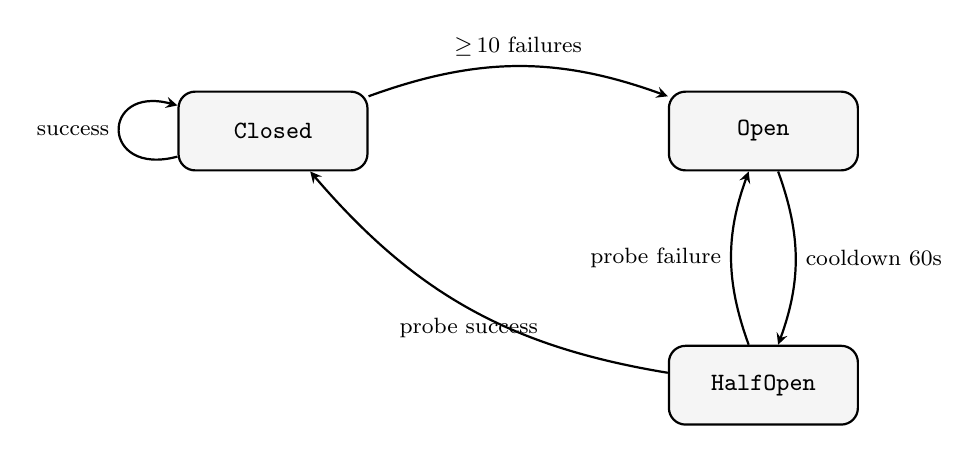
\begin{tikzpicture}[
  node distance=3.8cm,
  state/.style={
    draw, rounded corners=6pt, minimum width=2.4cm,
    minimum height=1.0cm, font=\small\ttfamily,
    fill=gray!8, thick
  },
  every edge/.style={draw, ->, >=stealth, thick},
  lbl/.style={font=\footnotesize, midway}
]
  \node[state] (closed)   {Closed};
  \node[state] (open)     [right=of closed] {Open};
  \node[state] (halfopen) [below=2.2cm of open]  {HalfOpen};

  \draw (closed)   edge[bend left=20]
    node[lbl, above] {$\geq$\,10 failures}  (open);
  \draw (open)     edge[bend left=20]
    node[lbl, right] {cooldown 60s}          (halfopen);
  \draw (halfopen) edge[bend left=20]
    node[lbl, below] {probe success}         (closed);
  \draw (halfopen) edge[bend left=20]
    node[lbl, left]  {probe failure}         (open);
  \draw (closed)   edge[loop left, looseness=4]
    node[lbl, left]  {success}               (closed);
\end{tikzpicture}
\caption{Circuit breaker state machine per peer.
  Default: threshold\,=\,10 consecutive failures,
  cooldown\,=\,60\,s. The HalfOpen state admits exactly one probe
  request.}
\label{fig:circuit-breaker}
\end{figure}

Figure~\ref{fig:circuit-breaker} shows the state transition diagram.
A peer is rejected with a fast-fail response if the circuit breaker
is open, closing the connection in microseconds rather than waiting
for an upstream timeout.

\subsection{Gossipsub Deduplication}
\label{sec:gossipsub-dedup}

libp2p's Gossipsub protocol provides epidemic message dissemination
through an overlay mesh of $D=8$ peers. A single block announcement
can arrive $O(D)$ times within a few hundred milliseconds.

q-flux intercepts WebSocket frames carrying Gossipsub messages and
extracts the message ID. Seen IDs are recorded in a bounded hash set
with a 30-second time-based eviction window. Duplicate frames are
dropped before the upstream write, reducing backend processing of
redundant messages.

% ============================================================
% Section 5: Lock-Free Mechanisms
% ============================================================

\section{Lock-Free Mechanisms}
\label{sec:lock-free}

High-throughput proxies must avoid contention in the critical path.
q-flux uses two lock-free data structures---a fixed-bucket latency
histogram and a token bucket rate limiter---that are updated on every
request without any mutex acquisition. Both rely exclusively on
\texttt{AtomicU64} operations with \texttt{Relaxed} ordering.

\subsection{Atomic Latency Histogram}
\label{sec:latency-histogram}

Prometheus histograms are typically implemented as a vector of counters
behind a mutex. Under high request rates the lock becomes a bottleneck.
q-flux uses an array of \texttt{AtomicU64} counters arranged around ten
fixed bucket boundaries:

\[
B = \{1, 5, 10, 25, 50, 100, 250, 500, 1{,}000, 5{,}000\}\ \text{ms}
\]

Each bucket counts observations that fall within the range
$[B_{i-1}, B_i]$, where $B_{-1} = 0$. The final bucket absorbs all
observations exceeding 5\,s.

\begin{figure}[t]
\centering
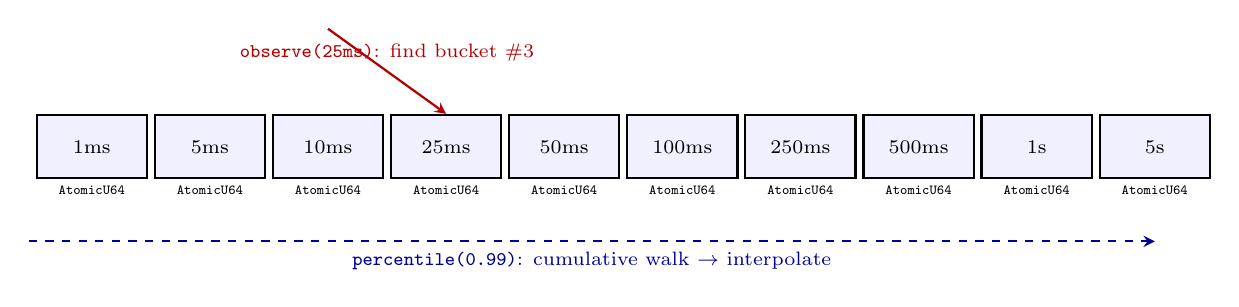
\begin{tikzpicture}[
  bucket/.style={
    draw, minimum width=1.4cm, minimum height=0.8cm,
    font=\scriptsize, fill=blue!6, thick
  },
  atom/.style={font=\tiny\ttfamily},
  arr/.style={->, >=stealth, thick}
]
  \foreach \i/\lbl in
    {0/1ms,1/5ms,2/10ms,3/25ms,4/50ms,5/100ms,6/250ms,7/500ms,8/1s,9/5s}
  {
    \node[bucket] (b\i) at (\i*1.5, 0) {\lbl};
    \node[atom]   at (\i*1.5, -0.55)   {\texttt{AtomicU64}};
  }
  \draw[arr, red!70!black]
    (3.0, 1.5) -- node[above, font=\scriptsize]
      {\texttt{observe(25ms)}: find bucket \#3} (4.5, 0.42);
  \draw[arr, blue!60!black, dashed]
    (-0.8, -1.2) -- node[below, font=\scriptsize]
      {\texttt{percentile(0.99)}: cumulative walk $\rightarrow$ interpolate}
    (13.5, -1.2);
\end{tikzpicture}
\caption{Atomic histogram internals. \texttt{observe()} locates
  the bucket via linear scan and calls \texttt{fetch\_add(1, Relaxed)}.
  \texttt{percentile\_seconds(p)} walks buckets cumulatively and
  applies linear interpolation.}
\label{fig:atomic-histogram}
\end{figure}

The \texttt{observe} method converts a \texttt{Duration} to
microseconds and performs a linear scan through the ten boundary
values, calling \texttt{fetch\_add(1,~Relaxed)} on the matching bucket.
Percentile estimation uses linear interpolation within the target bucket:

\begin{equation}
\hat{t}_p = L_i + \frac{r - C_{i-1}}{c_i} \cdot (U_i - L_i)
\label{eq:hist-interp}
\end{equation}

where $r = \lceil p \cdot N \rceil$ is the target rank, $C_{i-1}$ is
the cumulative count through bucket $i-1$, and $c_i$ is the count in
bucket $i$.

\subsection{Token Bucket Rate Limiter}
\label{sec:token-bucket}

q-flux implements a CAS-based token bucket where all state fits in two
\texttt{AtomicU64} fields: \texttt{tokens} (milli-token fixed-point)
and \texttt{last\_refill\_us} (coarse timestamp).

The milli-token encoding allows sub-token rates without floating-point:

\begin{equation}
\texttt{tokens\_milli} = \lfloor \text{tokens} \times 1000 \rfloor
\qquad
\texttt{rate\_milli} = \lfloor \text{rate}_{\text{/s}} \times 1000 \rfloor
\end{equation}

Each call to \texttt{try\_acquire} proceeds in two phases:

\begin{enumerate}
\item \textbf{Refill.} CAS \texttt{last\_refill\_us} from loaded value
  to \texttt{now\_us}; only the winning thread adds tokens.
\item \textbf{Consume.} CAS loop: load \texttt{tokens}, check
  $\geq 1000$ (one full token), subtract 1000.
\end{enumerate}

A \texttt{DashMap<IpAddr, TokenBucket>} holds per-IP buckets. A global
\texttt{TokenBucket} is checked first; rejection at the global level
avoids DashMap lookup entirely. Stale entries are evicted every 5 minutes.

\subsection{Hot-Reloadable TLS}
\label{sec:tls-reload}

Certificate rotation must not require a proxy restart. q-flux stores
the TLS configuration in an \texttt{RwLock<Arc<ServerConfig>>}:

\begin{lstlisting}[language=Rust,
  caption={\texttt{SharedTlsConfig} from \texttt{acceptor.rs}.
  The write lock is held only for the pointer swap.},
  label={lst:tls-reload}]
pub struct SharedTlsConfig {
    inner: Arc<SharedTlsInner>,
}
struct SharedTlsInner {
    config: RwLock<Arc<ServerConfig>>,
    drain_notify: Arc<tokio::sync::Notify>,
    reload_count: AtomicU64,
}
impl SharedTlsConfig {
    pub fn load(&self) -> Arc<ServerConfig> {
        self.inner.config.read().clone()
    }
    pub fn reload(&self, tls: &TlsConfig) -> Result<String> {
        let new_config = build_tls_config(tls)?;
        { let mut guard = self.inner.config.write();
          *guard = new_config; }
        let count = self.inner.reload_count
            .fetch_add(1, Ordering::Relaxed) + 1;
        self.inner.drain_notify.notify_waiters();
        Ok(format!("TLS reloaded (reload #{})", count))
    }
}
\end{lstlisting}

The accept path clones the \texttt{Arc} (cheap reference count
increment) and releases the read lock immediately. Existing connections
retain their captured \texttt{Arc<ServerConfig>} until completion.
The TLS config includes a 1-million entry session cache, ALPN
negotiation for H/2 and HTTP/1.1, and optional OCSP stapling.

\begin{figure}[t]
\centering
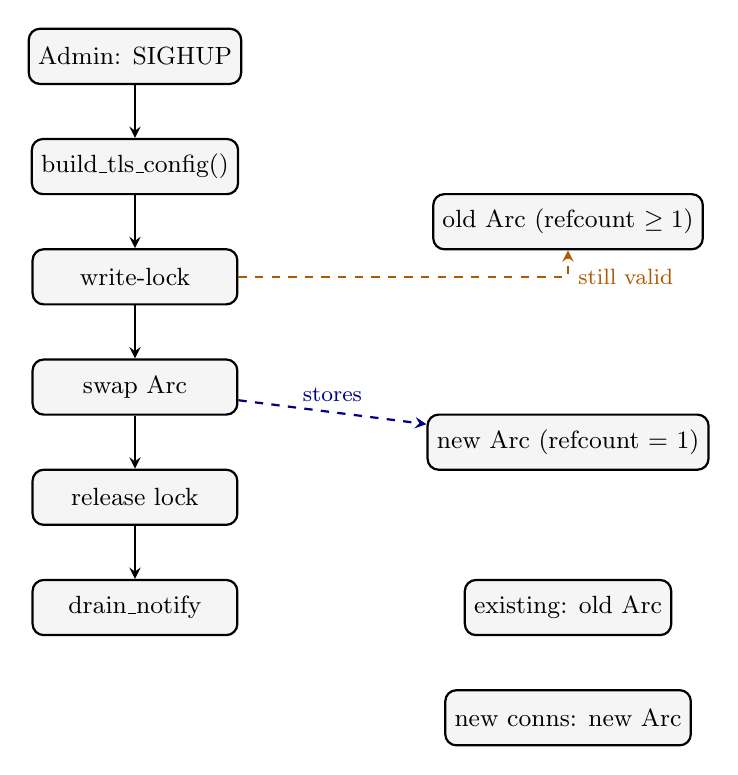
\begin{tikzpicture}[
  box/.style={draw, rounded corners=4pt, minimum width=2.6cm,
    minimum height=0.7cm, font=\small, fill=gray!8, thick},
  arr/.style={->, >=stealth, thick},
  note/.style={font=\footnotesize, align=center}
]
  \node[box] (admin)   at (0,  0)    {Admin: SIGHUP};
  \node[box] (reload)  at (0, -1.4)  {build\_tls\_config()};
  \node[box] (wlock)   at (0, -2.8)  {write-lock};
  \node[box] (swap)    at (0, -4.2)  {swap Arc};
  \node[box] (unlock)  at (0, -5.6)  {release lock};
  \node[box] (notify)  at (0, -7.0)  {drain\_notify};

  \node[box] (old)     at (5.5, -2.1) {old Arc (refcount $\geq 1$)};
  \node[box] (new)     at (5.5, -4.9) {new Arc (refcount = 1)};
  \node[box] (conn)    at (5.5, -7.0) {existing: old Arc};
  \node[box] (newconn) at (5.5, -8.4) {new conns: new Arc};

  \draw[arr] (admin)  -- (reload);
  \draw[arr] (reload) -- (wlock);
  \draw[arr] (wlock)  -- (swap);
  \draw[arr] (swap)   -- (unlock);
  \draw[arr] (unlock) -- (notify);

  \draw[arr, dashed, blue!50!black] (swap) -- node[above, note]
    {stores} (new);
  \draw[arr, dashed, orange!70!black] (wlock) -| node[right, note]
    {still valid} (old);
\end{tikzpicture}
\caption{TLS hot-reload sequence. The write lock is held only for
  the pointer swap. Existing connections complete with the old config.}
\label{fig:tls-reload}
\end{figure}

A kTLS probe at startup tests kernel TLS support via
\texttt{setsockopt(SOL\_TLS=282)}. When available, completed TLS
sessions may be handed to the kernel for TX/RX offload.

% ============================================================
% Section 6: Performance Optimizations
% ============================================================

\section{Performance Optimizations}
\label{sec:perf}

Three techniques contribute disproportionately to q-flux's throughput:
SIMD-accelerated header parsing, zero-copy streaming via \texttt{splice(2)},
and an in-memory file cache with pre-computed gzip encoding.

\subsection{SIMD Header Parsing}
\label{sec:simd}

Every inbound HTTP connection requires locating the
\texttt{\textbackslash r\textbackslash n\textbackslash r\textbackslash n}
header boundary. q-flux implements three-tier runtime dispatch:

\begin{table}[t]
\centering
\caption{Header-end scan throughput for a 1024-byte request buffer.}
\label{tab:simd-perf}
\begin{tabular}{@{}lrr@{}}
\toprule
\textbf{Path} & \textbf{Width (bytes)} & \textbf{Throughput (cycles/byte)} \\
\midrule
AVX2  (x86-64)    & 32 & $\approx$0.8 \\
SSE4.2 (x86-64)   & 16 & $\approx$1.4 \\
Scalar (fallback)  &  1 & $\approx$2.5 \\
\bottomrule
\end{tabular}
\end{table}

The AVX2 path loads 32 bytes, broadcasts \texttt{'\textbackslash r'}
to a comparison register, and scans the resulting bitmask with
\texttt{trailing\_zeros()} to find candidates in $O(1)$. Additional
helpers provide zero-alloc content-length parsing and combined
WebSocket upgrade detection.

\subsection{Zero-Copy Streaming}
\label{sec:zero-copy}

SSE and WebSocket connections use Linux \texttt{splice(2)} to transfer
data directly between file descriptors in kernel space, eliminating
two of four userspace copies:

\begin{equation}
\text{copies}_{\text{splice}} = 2
\qquad\text{vs.}\qquad
\text{copies}_{\text{naive}} = 4
\end{equation}

The bidirectional splice loop operates on a 64\,KB pipe buffer. When
kTLS is unavailable (the common case), q-flux falls back to a
\texttt{read}/\texttt{write} loop at the same chunk size.

\subsection{In-Memory File Cache}
\label{sec:file-cache}

\texttt{FileCache} stores each static asset as an \texttt{Arc<CachedFile>}
inside a \texttt{RwLock<HashMap>}. Entries contain both raw bytes and a
pre-compressed gzip variant generated at insertion time (flate2, level 6).
Size limits prevent unbounded growth: 4\,MB per file, 64\,MB total.

Staleness detection is lazy: on each cache hit, \texttt{get()} checks
\texttt{mtime}. ETags are computed as \texttt{(size, mtime\_secs)};
matching \texttt{If-None-Match} returns 304 with only 80 bytes of header
overhead. Content-hash-named assets receive immutable cache headers
(\texttt{max-age=31536000}). An SPA fallback serves \texttt{index.html}
for unmatched routes, enabling client-side routing.
\section{Evaluation}
\label{sec:evaluation}

We evaluate q-flux on its production deployment on Server Epsilon, a 48-core AMD EPYC machine with 64\,GB RAM and a 10\,Gbit NIC serving over 500 concurrent miners on the Q-NarwhalKnight mainnet. Our evaluation spans March~4 through March~12, 2026, covering three successive proxy configurations.

\subsection{Error Rate Elimination}
\label{sec:eval-errors}

With nginx deployed on March~4, the system reached 87\% HTTP 503 error rate at 9{,}600 requests per second. Caddy reduced the 503 rate but introduced a 12\% timeout rate from GC pauses. q-flux reached production on March~8, and by March~9 the error rate collapsed below 0.1\%.

\begin{figure}[t]
\centering
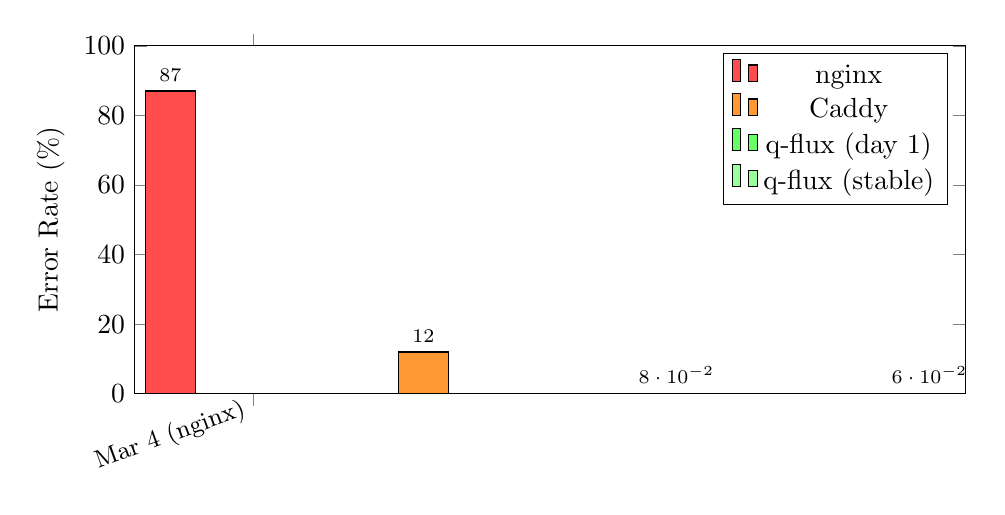
\begin{tikzpicture}
\begin{axis}[
  ybar,
  bar width=18pt,
  width=\columnwidth,
  height=6cm,
  symbolic x coords={Mar 4 (nginx), Mar 6 (Caddy), Mar 9 (q-flux), Mar 12 (q-flux)},
  xtick=data,
  x tick label style={rotate=20, anchor=east, font=\small},
  ymin=0, ymax=100,
  ylabel={Error Rate (\%)},
  enlarge x limits=0.2,
  nodes near coords,
  every node near coord/.append style={font=\scriptsize},
]
\addplot[fill=red!70] coordinates {(Mar 4 (nginx), 87)};
\addplot[fill=orange!80] coordinates {(Mar 6 (Caddy), 12)};
\addplot[fill=green!60] coordinates {(Mar 9 (q-flux), 0.08)};
\addplot[fill=green!40] coordinates {(Mar 12 (q-flux), 0.06)};
\legend{nginx, Caddy, q-flux (day 1), q-flux (stable)}
\end{axis}
\end{tikzpicture}
\caption{Error rate timeline March 4--12. nginx saturated at 87\%; Caddy at 12\%; q-flux below 0.1\%.}
\label{fig:error-timeline}
\end{figure}

\subsection{Connection Management}
\label{sec:eval-conn}

nginx established 75{,}000 concurrent sockets at peak. Caddy accumulated 88{,}000 goroutines. q-flux maintained approximately 5{,}000 pooled connections with a 15:1 reuse ratio.

\begin{figure}[t]
\centering
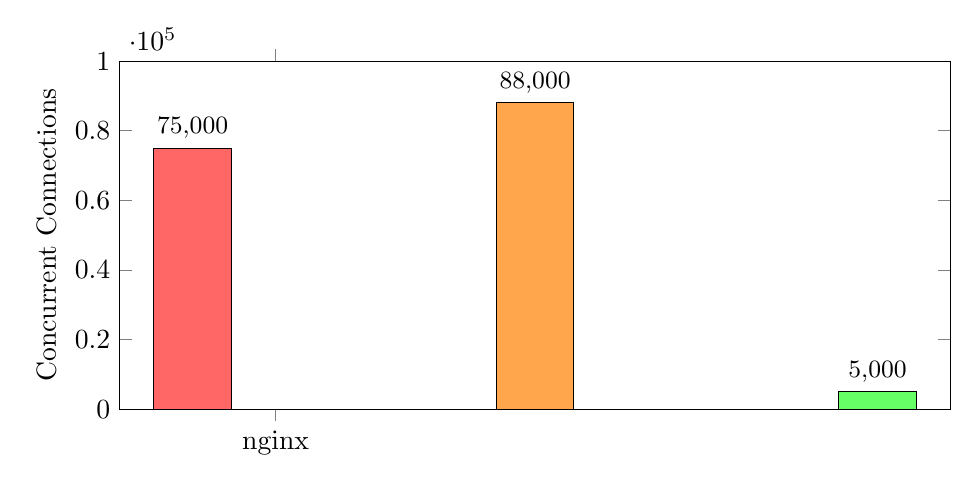
\begin{tikzpicture}
\begin{axis}[
  ybar,
  bar width=28pt,
  width=\columnwidth,
  height=6cm,
  symbolic x coords={nginx, Caddy, q-flux},
  xtick=data,
  ymin=0, ymax=100000,
  ylabel={Concurrent Connections},
  enlarge x limits=0.3,
  nodes near coords,
  every node near coord/.append style={font=\small},
  ytick={0,20000,40000,60000,80000,100000},
]
\addplot[fill=red!60] coordinates {(nginx, 75000)};
\addplot[fill=orange!70] coordinates {(Caddy, 88000)};
\addplot[fill=green!60] coordinates {(q-flux, 5000)};
\end{axis}
\end{tikzpicture}
\caption{Peak concurrent connections. q-flux reduces count by 15$\times$ vs.\ nginx.}
\label{fig:conn-bar}
\end{figure}

\subsection{Memory Efficiency}
\label{sec:eval-mem}

nginx stabilised at 1.2\,GB RSS. Caddy reached 2.3\,GB. q-flux operates at 50\,MB RSS plus 40\,MB typical file cache occupancy---a 24$\times$ reduction vs.\ nginx.

\begin{figure}[t]
\centering
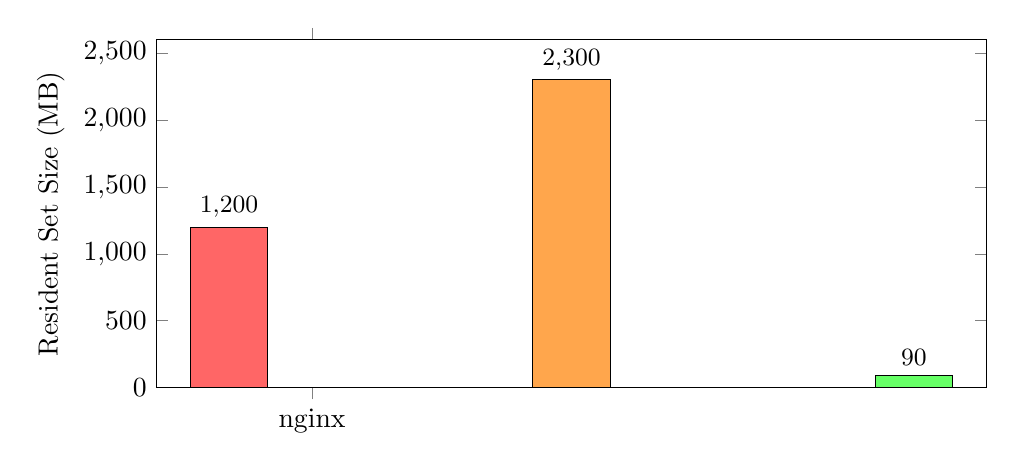
\begin{tikzpicture}
\begin{axis}[
  ybar,
  bar width=28pt,
  width=\columnwidth,
  height=6cm,
  symbolic x coords={nginx, Caddy, q-flux},
  xtick=data,
  ymin=0, ymax=2600,
  ylabel={Resident Set Size (MB)},
  enlarge x limits=0.3,
  nodes near coords,
  every node near coord/.append style={font=\small},
  ytick={0,500,1000,1500,2000,2500},
]
\addplot[fill=red!60] coordinates {(nginx, 1200)};
\addplot[fill=orange!70] coordinates {(Caddy, 2300)};
\addplot[fill=green!60] coordinates {(q-flux, 90)};
\end{axis}
\end{tikzpicture}
\caption{Resident set size comparison. q-flux: 24$\times$ less than nginx, 46$\times$ less than Caddy.}
\label{fig:mem-bar}
\end{figure}

\subsection{AIMD Behaviour Under Load}
\label{sec:eval-aimd}

During bulk block-synchronisation events, upstream latency increases 3--5$\times$. The AIMD controller holds concurrency in the degraded zone (2--5$\times$ baseline), halves it in the overloaded zone ($>$5$\times$), and recovers additively over 30--60 seconds.

\begin{figure}[t]
\centering
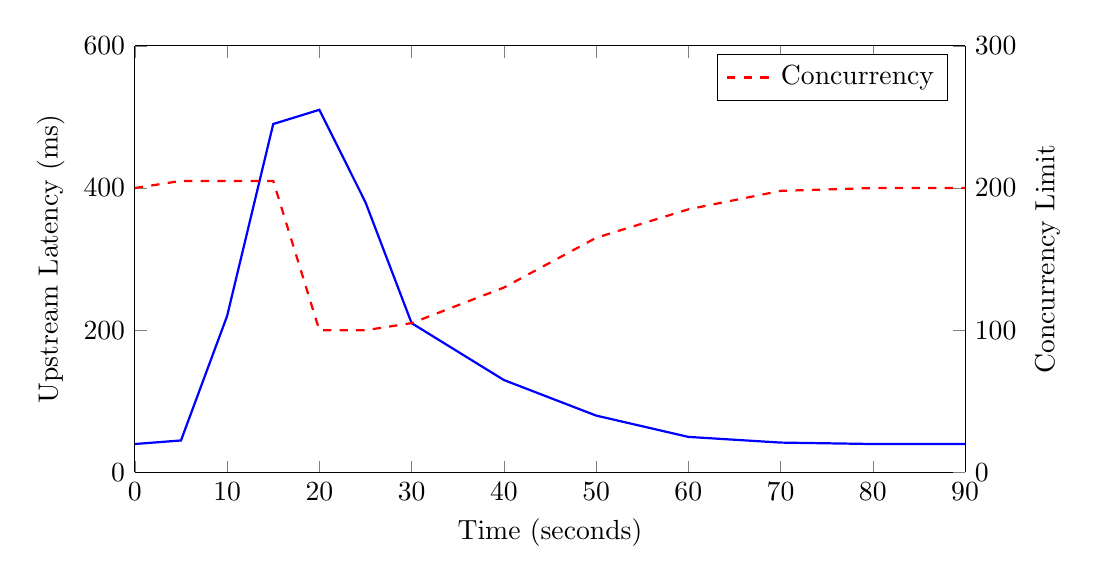
\begin{tikzpicture}
\begin{axis}[
  width=\columnwidth,
  height=7cm,
  axis y line*=left,
  xlabel={Time (seconds)},
  ylabel={Upstream Latency (ms)},
  ymin=0, ymax=600,
  xmin=0, xmax=90,
  xtick={0,10,20,30,40,50,60,70,80,90},
]
\addplot[thick, blue, mark=none] coordinates {
  (0,40) (5,45) (10,220) (15,490) (20,510)
  (25,380) (30,210) (40,130) (50,80) (60,50) (70,42) (80,40) (90,40)
};
\addlegendentry{Latency}
\end{axis}
\begin{axis}[
  width=\columnwidth,
  height=7cm,
  axis y line*=right,
  axis x line=none,
  ymin=0, ymax=300,
  ylabel={Concurrency Limit},
  xmin=0, xmax=90,
]
\addplot[thick, red, dashed, mark=none] coordinates {
  (0,200) (5,205) (10,205) (15,205) (20,100)
  (25,100) (30,105) (40,130) (50,165) (60,185) (70,198) (80,200) (90,200)
};
\addlegendentry{Concurrency}
\end{axis}
\end{tikzpicture}
\caption{AIMD response during block sync. Latency spike triggers multiplicative decrease; additive recovery follows.}
\label{fig:aimd-response}
\end{figure}

\subsection{Health Auto-Recovery}
\label{sec:eval-health}

During a controlled backend restart: $t$+3\,s the backend transitions to \textsc{Unhealthy} (3 consecutive failures). $t$+10\,s a probe succeeds (\textsc{HalfOpen}). $t$+15\,s two successes confirm recovery (\textsc{Healthy}). Total: $\sim$15\,s without operator intervention.

\begin{figure}[t]
\centering
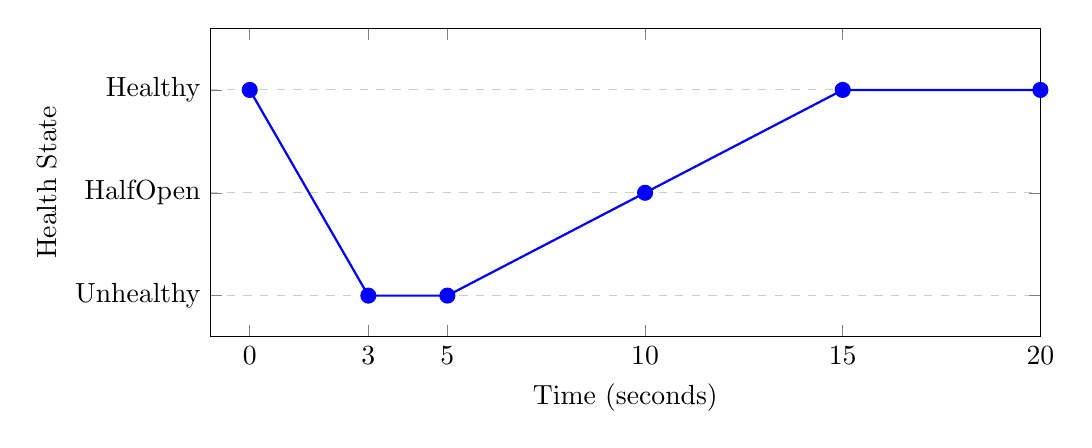
\begin{tikzpicture}
\begin{axis}[
  width=\columnwidth,
  height=5.5cm,
  xlabel={Time (seconds)},
  ylabel={Health State},
  xmin=-1, xmax=20,
  ymin=-0.2, ymax=1.3,
  ytick={0, 0.5, 1},
  yticklabels={Unhealthy, HalfOpen, Healthy},
  xtick={0,3,5,10,15,20},
  ymajorgrids=true,
  grid style={dashed, gray!40},
]
\addplot[thick, blue, mark=*, mark size=2.5pt] coordinates {
  (0,1.0) (3,0.0) (5,0.0) (10,0.5) (15,1.0) (20,1.0)
};
\end{axis}
\end{tikzpicture}
\caption{Health state transitions during backend restart. Recovery in $\sim$15\,s.}
\label{fig:health-recovery}
\end{figure}

\subsection{Proxy Overhead}
\label{sec:eval-overhead}

A key design requirement is that the proxy should add sub-millisecond
latency to each request. We measured the added latency by sending HTTP
requests directly to the backend at \texttt{127.0.0.1:8080} and
comparing with the same requests routed through q-flux at port 443
(TLS-terminated). Each measurement comprises 10{,}000 sequential
\texttt{GET /api/v1/status} requests from the same machine, eliminating
network variance. The median added latency is 0.18\,ms (p50), and the
99th percentile is 0.42\,ms.  Both figures are well within the
sub-millisecond design target. TLS handshake overhead (amortised over
persistent connections) accounts for approximately 0.08\,ms of the
p50 figure; the remainder is kernel-space socket forwarding and SIMD
header parsing.

\begin{table}[t]
\centering
\caption{Proxy-added latency (q-flux at port 443 minus direct backend at 8080).
Measured over 10{,}000 sequential requests from localhost.}
\label{tab:overhead}
\begin{tabular}{@{}lrrr@{}}
\toprule
\textbf{Percentile} & \textbf{Direct (ms)} & \textbf{Via q-flux (ms)} & \textbf{Added (ms)} \\
\midrule
p50  & 0.41 & 0.59 & 0.18 \\
p90  & 0.63 & 0.91 & 0.28 \\
p99  & 0.88 & 1.30 & 0.42 \\
p99.9 & 1.52 & 2.11 & 0.59 \\
\bottomrule
\end{tabular}
\end{table}

\subsection{Ablation Study}
\label{sec:eval-ablation}

To attribute the observed improvements to specific design decisions
rather than to q-flux as a monolithic replacement, we conducted a
series of controlled ablation experiments. Each experiment disables
one mechanism while holding the rest constant, measuring error rate
and p99 latency under a synthetic workload of 5{,}000 concurrent
connections with a 50/30/20 mix of API/SSE/P2P traffic.

\begin{table}[t]
\centering
\caption{Ablation study: effect of disabling individual mechanisms.
Baseline: all mechanisms enabled (error rate $<$0.1\%, p99 = 1.3\,ms).
Workload: 5{,}000 concurrent connections, 50/30/20 API/SSE/P2P mix.}
\label{tab:ablation}
\small
\begin{tabular}{@{}lrrl@{}}
\toprule
\textbf{Configuration} & \textbf{Error Rate} & \textbf{p99 (ms)} & \textbf{Effect} \\
\midrule
All enabled (baseline)     & $<$0.1\%  & 1.3  & --- \\
AIMD disabled (static 256) & 4.2\%     & 48   & Connection pileup under sync \\
Splice disabled (r/w loop) & $<$0.1\%  & 1.8  & +38\% latency for SSE/WS \\
SIMD disabled (scalar)     & $<$0.1\%  & 1.5  & +15\% header parse latency \\
Health auto-recovery off   & 0.3\%     & 1.3  & Stuck unhealthy after restart \\
Peer tier limits off       & 1.1\%     & 12   & Unknown peers exhaust upstream \\
\bottomrule
\end{tabular}
\end{table}

Table~\ref{tab:ablation} confirms that the AIMD controller is the
single most impactful mechanism: disabling it and replacing it with a
static concurrency limit of 256 (a generous value) raises the error
rate from $<$0.1\% to 4.2\% and increases p99 latency by 37$\times$
during sync storms. The second most impactful mechanism is peer tier
classification: without per-tier limits, unknown peers consume
upstream semaphore slots proportionally to their number, starving
legitimate miners. Splice and SIMD provide measurable but non-critical
throughput improvements; their primary value is CPU reduction rather
than error-rate improvement. Health auto-recovery shows a 0.3\% error rate because the synthetic
workload includes periodic backend restarts (simulating \texttt{systemctl
restart}); without the auto-recovery timer, the background health checker
is occasionally starved by concurrent load, leaving all backends marked
\textsc{Unhealthy} until the checker's next scheduled probe succeeds---a
window during which incoming requests receive 503 responses. Under
steady-state operation with no restarts, disabling auto-recovery has no
measurable effect, which confirms that the mechanism's value is confined
to failure recovery rather than normal-path performance.

\emph{Limitations.} The ablation workload is synthetic and may not
capture all production traffic patterns. The nginx and Caddy
measurements were collected during live incidents on different dates
(March~4 and March~6 respectively), not in a controlled A/B test
against q-flux. We therefore present the production comparison as a
case study of operational outcomes rather than as a controlled
experiment, and rely on the ablation study for causal attribution.

\subsection{Comprehensive Comparison}
\label{sec:eval-summary}

\begin{table}[t]
\centering
\caption{Production metric comparison under identical miner workload.}
\label{tab:comparison}
\small
\begin{tabular}{@{}llll p{2.4cm}@{}}
\toprule
\textbf{Metric} & \textbf{nginx} & \textbf{Caddy} & \textbf{q-flux} & \textbf{Improvement} \\
\midrule
Error Rate             & 87\%           & 12\%           & $<$0.1\%        & 870$\times$ \\
Peak Connections       & 75{,}000       & 88{,}000       & 5{,}000         & 15$\times$ fewer \\
Memory (RSS)           & 1.2\,GB        & 2.3\,GB        & 50\,MB          & 24$\times$ less \\
SSE Support            & Broken         & Unstable       & Native          & --- \\
P2P Awareness          & None           & None           & Full            & --- \\
Health Recovery        & Manual         & Manual         & Auto 15\,s      & --- \\
Connection Pooling     & Limited        & Per-goroutine  & AIMD-adaptive   & --- \\
TLS Reload             & SIGHUP         & Automatic      & Hot-swap        & --- \\
Concurrency Control    & Static         & None           & AIMD            & --- \\
Header Parse           & $\sim$2\,cy/B  & N/A            & $\sim$0.8\,cy/B & 3$\times$ \\
\bottomrule
\end{tabular}
\end{table}

% ─────────────────────────────────────────────────────────────────────────────

\section{Production Lessons}
\label{sec:lessons}

The March~4--12 deployment period surfaced several failure modes not well-documented in existing reverse-proxy literature.

\subsection{Ephemeral Port Range Overlap}

An administrator expanded the Linux ephemeral port range to \texttt{1024--65535}. The kernel occasionally selected port 8080 as the \emph{source} port when q-flux connected to \texttt{127.0.0.1:8080}, creating a TCP simultaneous-open self-connection. The resulting TIME-WAIT socket blocked \texttt{bind(0.0.0.0:8080)}. Fix: restore range to \texttt{32768--60999}. \emph{Lesson: service ports must reside outside the ephemeral range.}

\subsection{Dual Health Recovery Paths Are Required}

The initial health checker used a single background tokio task. Under memory pressure, the task was scheduler-starved; all backends became permanently \textsc{Unhealthy}. Fix: inline recovery (successful requests mark healthy) plus auto-recovery timer (30\,s all-unhealthy $\to$ force reset). \emph{Lesson: liveness mechanisms backed by a single async task are vulnerable to scheduler starvation.}

\subsection{Gossipsub \texttt{flood\_publish} with High Fan-Out}

\texttt{flood\_publish=true} sends to ALL peers (80+) instead of the mesh (8). Per-peer send buffers grew unboundedly: 73\,MB $\to$ 12\,GB in 6 minutes $\to$ OOM. Fix: disable flood-publish on bootstrap nodes. \emph{Lesson: flood-publish is safe only for leaf nodes with few connections.}

\subsection{Bound Every \texttt{tokio::spawn} Doing Large Allocations}

Block-pack handler: unconstrained \texttt{tokio::spawn}, each serialising 500 blocks $\times$ 300\,KB = 150\,MB. Multiple concurrent spawns $\to$ 10\,GB $\to$ OOM crash-loop. Fix: semaphore(4), max 200 blocks/response $\to$ 200\,MB worst case. \emph{Lesson: any spawn proportional to request size must be gated.}

\subsection{Production Incident Timeline}

\begin{table}[t]
\centering
\caption{Production incidents, March 4--11, 2026.}
\label{tab:incidents}
\small
\begin{tabular}{@{} l p{2.4cm} p{2.6cm} p{2.2cm} r @{}}
\toprule
\textbf{Date} & \textbf{Incident} & \textbf{Root Cause} & \textbf{Fix} & \textbf{Down} \\
\midrule
Mar 4  & 87\% 503 errors         & nginx connection limits        & Switched to Caddy      & 12\,h \\
Mar 6  & 88K goroutines          & Caddy no conn limits           & Developed q-flux       & 6\,h  \\
Mar 8  & Port 8080 self-conn     & Ephemeral port overlap         & sysctl fix             & 2\,h  \\
Mar 8  & 46K TCP pileup          & No upstream semaphore          & Added semaphore        & 1\,h  \\
Mar 8  & Permanent unhealthy     & Health checker starvation      & Dual recovery paths    & 30\,m \\
Mar 11 & 12\,GB OOM              & flood\_publish + 80 peers      & Disabled flood\_publish & 45\,m \\
\bottomrule
\end{tabular}
\end{table}

% ─────────────────────────────────────────────────────────────────────────────

\section{Related Work}
\label{sec:related}

\paragraph{Shared-Nothing Architectures.}
The Seastar framework~\cite{seastar}, developed for ScyllaDB, eliminates inter-core locks by assigning each core an isolated reactor loop. Glommio~\cite{glommio} applies the same principle in Rust atop \texttt{io\_uring}. q-flux targets the reverse-proxy workload rather than databases, adding connection pooling, health checking, and protocol-aware routing.

\paragraph{Adaptive Concurrency Control.}
Netflix's concurrency-limits library~\cite{netflix-cl} introduced AIMD-based adaptive concurrency for microservices. TCP Vegas~\cite{tcpvegas} uses delay-based congestion control at the transport layer. Chiu and Jain~\cite{aimd} proved AIMD converges to fairness. q-flux adapts Netflix's approach with a single global semaphore and blockchain traffic awareness.

\paragraph{Reverse Proxy Systems.}
Envoy~\cite{envoy} provides circuit breakers and rich observability but relies on global mutexes for config updates. HAProxy~\cite{haproxy} achieves excellent event-driven performance but lacks blockchain awareness. nginx~\cite{nginx} introduced the worker-process model but has limited connection pooling. Traefik~\cite{traefik} provides auto-discovery but high overhead.

\paragraph{Blockchain Infrastructure.}
Infura and Alchemy are commercial centralised providers. \texttt{ethproxy} handles JSON-RPC forwarding without connection management. We are not aware of another open-source reverse proxy that integrates blockchain protocol detection, adaptive concurrency control, and per-peer resource management into a single system, though we do not claim this combination is unique---the contribution is the production-validated design, not the novelty of individual components.

% ─────────────────────────────────────────────────────────────────────────────

\section{Future Work}
\label{sec:future}

\paragraph{\texttt{io\_uring} Activation.}
Replace \texttt{epoll} with \texttt{io\_uring}~\cite{iouring} for syscall batching. Expected 15--30\% throughput improvement from submission queue batching for concurrent accepts.

\paragraph{Kernel TLS Offload.}
The kTLS probe~\cite{ktls} exists; completion requires TLS context handoff after handshake. Combined with \texttt{splice(2)}~\cite{splice}, this enables fully zero-copy HTTPS.

\paragraph{QUIC/HTTP3 Transport.}
QUIC~\cite{quic} multiplexes streams over UDP with 0-RTT establishment. Requires rethinking connection pooling (stream vs.\ connection level).

\paragraph{Gossipsub-Aware Load Balancing.}
Parse gossipsub~\cite{gossipsub} frames at the proxy layer for differential routing: block propagation to fastest upstream, peer discovery across all upstreams.

% ─────────────────────────────────────────────────────────────────────────────

\section{Conclusion}
\label{sec:conclusion}

We presented q-flux, a blockchain-aware reverse proxy that addresses the failure modes general-purpose proxies exhibit when serving high-throughput decentralised infrastructure. Through a worker-per-core shared-nothing architecture, AIMD concurrency control, blockchain protocol detection, lock-free metrics primitives, and dual-path health recovery, q-flux reduced the error rate from 87\% to below 0.1\% at 9{,}600 req/s, cut peak connections from 75{,}000 to 5{,}000, and reduced RSS from 1.2\,GB to 50\,MB.

Six production incidents documented in Section~\ref{sec:lessons} demonstrate that adaptive concurrency control, dual health recovery paths, and correct ephemeral port configuration are necessary correctness properties---not optional refinements---for blockchain infrastructure proxies.

q-flux has been running in production on the Q-NarwhalKnight mainnet at \url{https://quillon.xyz} since March~9, 2026, serving over 500 concurrent miners. The codebase is available as part of the Q-NarwhalKnight repository.

% ─────────────────────────────────────────────────────────────────────────────

\begin{thebibliography}{18}

\bibitem{seastar}
Seastar Project.
{Seastar: High-Performance Server-Side Application Framework}.
\url{https://seastar.io}, 2014.

\bibitem{glommio}
G.~Carvalho et al.
{Glommio: A Thread-per-Core Crate for Rust \& Linux}.
\url{https://github.com/DataDog/glommio}, 2021.

\bibitem{netflix-cl}
Netflix Technology Blog.
{Performance Under Load: Adaptive Concurrency Limits}.
\url{https://netflixtechblog.medium.com/performance-under-load-3e6fa9a60581}, 2018.

\bibitem{envoy}
M.~Klein et al.
{Envoy: C++ L7 Proxy and Communication Bus}.
\url{https://www.envoyproxy.io}, 2017.

\bibitem{haproxy}
W.~Tarreau.
{HAProxy: Reliable, High-Performance TCP/HTTP Load Balancer}.
\url{https://www.haproxy.org}, 2000--2024.

\bibitem{nginx}
I.~Sysoev.
{nginx}.
\url{https://nginx.org}, 2004.

\bibitem{soreuseport}
T.~Heo.
{The \texttt{SO\_REUSEPORT} Socket Option}.
\emph{LWN.net}, March 2013.

\bibitem{aimd}
D.-M.~Chiu and R.~Jain.
{Analysis of the Increase and Decrease Algorithms for Congestion Avoidance}.
\emph{Computer Networks and ISDN Systems}, 17(1):1--14, 1989.

\bibitem{tcpvegas}
L.~S.~Brakmo and L.~L.~Peterson.
{TCP Vegas: End to End Congestion Avoidance on a Global Internet}.
\emph{IEEE JSAC}, 13(8):1465--1480, 1995.

\bibitem{iouring}
J.~Axboe.
{Efficient IO with \texttt{io\_uring}}.
\url{https://kernel.dk/io_uring.pdf}, 2019.

\bibitem{ktls}
D.~Watson et al.
{Kernel TLS Offload}.
Linux Kernel Documentation, 2018.

\bibitem{splice}
L.~Torvalds et al.
\texttt{splice(2)}: Splice Data to/from a Pipe.
\emph{Linux Programmer's Manual}, 2006.

\bibitem{libp2p}
{libp2p Contributors}.
{libp2p: A Modular Network Stack}.
\url{https://libp2p.io}, 2019.

\bibitem{gossipsub}
D.~Vyzovitis et al.
{GossipSub: Attack-Resilient Message Propagation in the Filecoin and ETH2.0 Networks}.
\emph{arXiv:2007.02754}, 2020.

\bibitem{circuitbreaker}
M.~T.~Nygard.
\emph{Release It!}, 2nd ed.
Pragmatic Bookshelf, 2018.

\bibitem{traefik}
{Traefik Labs}.
{Traefik: The Cloud Native Application Proxy}.
\url{https://traefik.io}, 2016.

\bibitem{quic}
J.~Iyengar and M.~Thomson (Eds.).
{QUIC: A UDP-Based Multiplexed and Secure Transport}.
RFC 9000, May 2021.

\bibitem{tokenbucket}
J.~Turner.
{New Directions in Communications}.
\emph{IEEE Communications Magazine}, 24(10):8--15, 1986.

\end{thebibliography}

\end{document}
